\documentclass[11pt]{article}
\usepackage{vntex}
\usepackage[english]{babel}
\usepackage[utf8]{inputenc}
\usepackage[colorlinks = true,
            linkcolor = blue,
            urlcolor  = blue]{hyperref}
\usepackage[a4paper,margin=1.5in]{geometry}
\usepackage{stackengine,graphicx}
\usepackage{fancyhdr}
\setlength{\headheight}{15pt}
\usepackage{microtype}
\usepackage{times}
\usepackage{booktabs}
\usepackage{gensymb}
\usepackage{amsmath, amsfonts, bbm, amssymb, isomath}
\usepackage{float}


% \setmathfontface\mymathit{FreeSansOblique}
% \DeclareMathAlphabet{\mathit}{T1}{\sfdefault}{\mddefault}{\sldefault}
% \SetMathAlphabet{\mathit}{bold}{T1}{\sfdefault}{\bfdefault}{\sldefault}

% python code format: https://github.com/olivierverdier/python-latex-highlighting
\usepackage{pythonhighlight}

\frenchspacing
\setlength{\parindent}{0cm} % Default is 15pt.
\setlength{\parskip}{0.3cm plus1mm minus1mm}

\pagestyle{fancy}
\fancyhf{}
\lhead{Bài tập lớn 3}
\rhead{Xử lý ảnh số và thị giác máy tính}
\rfoot{\thepage}

\date{}

\title{\vspace{-1cm}Bài tập lớn 3: Camera Calibration and Fundamental Matrix Estimation with RANSAC}

\setcounter{MaxMatrixCols}{20}

\begin{document}
\maketitle
\vspace{-2cm}
\thispagestyle{fancy}

\section*{Giới thiệu}
Nhận dạng và so trùng đặc trưng giữa hai ảnh được thực hiện bằng các xác định các điểm góc (corner points), và khớp các đặc trưng xung quanh các điểm góc đó. Các giải thuật như SFIT (thực hiện trong bài tập lớn 2) phụ thuộc vào gradient của pixel xung quanh điểm góc, nên rất nhạy cảm với các hiệu chỉnh thông số bên ngoài như camera calibration. Vì vậy, nếu camera được xoay để chụp một vật thể ở một góc khác, SIFT sẽ cho kết quả rất kém.

Vì vậy, trong bài tập lớn này sẽ yêu cầu tính toán các thông số bên ngoài như vị trí máy ảnh, tỷ lệ khung hình, độ lệch giữa các trục dựa vào các mối tương quan hình học giữa các hình ảnh được chụp từ nhiều góc chụp khác nhau.

Bài tập lớn được chia làm 3 phần:
\begin{itemize}
    \item Phần 1: Tính toán ma trận Camera Projection Matrix (M) dựa vào các cặp điểm tương ứng trong không gian ảnh 2D và không gian thế giới thực 3D, sau đó tính toán camera's center dựa vào ma trận M.
    \item Phần 2: Tính toán ma trận Fundamental Matrix dựa vào các cặp điểm tương ứng trên 2 ảnh.
    \item Phần 3: Hiện thực giải thuật RANSAC (Random sample consensus) để tính toán ma trận Fundamental Matrix
\end{itemize}

\section*{Camera Projection Matrix}

\subsection*{Chi tiết hiện thực}

Projection matirix được sử dụng để chuyển đổi các điểm từ không gian thế giới thực 3D về không gian ảnh 2D.
\begin{equation*}
    \mathit{x} = \mathit{K} [\mathit{R} \; \mathit{t}] \mathit{X}
\end{equation*}
trong đó:
\begin{itemize}
    \item $\mathit{x}$: toạ độ trong không gian ảnh (u, v, 1)
    \item $\mathit{K}$: Intrinsic Matrix (3x3)
    \item $\mathit{R}$: Rotation (3x3)
    \item $\mathit{t}$: Translation (3x1)
    \item $\mathit{X}$: toạ độ trong không gian thế giới thực (X, Y, Z, 1)
\end{itemize}

\begin{align*} 
    \Leftrightarrow \mathit{w}
    \begin{bmatrix}
        \mathit{u} \\
        \mathit{v} \\
        1
    \end{bmatrix}
    = 
    \begin{bmatrix}
        \mathit{f}_\mathit{x} & \mathit{s} & \mathit{u}_0\\
        0  & \mathit{f}_\mathit{y} & \mathit{v}_0\\
        0 & 0 & 1
    \end{bmatrix}
    \begin{bmatrix}
        \mathit{r}_{11} & \mathit{r}_{12} & \mathit{r}_{13} & \mathit{t}_\mathit{x} \\
        \mathit{r}_{21} & \mathit{r}_{22} & \mathit{r}_{23} & \mathit{t}_\mathit{y} \\
        \mathit{r}_{31} & \mathit{r}_{32} & \mathit{r}_{33} & \mathit{t}_\mathit{z}
    \end{bmatrix}
    \begin{bmatrix}
        \mathit{X}\\
        \mathit{Y}\\
        \mathit{Z}\\
        1
    \end{bmatrix}
\end{align*}

\begin{align*} 
    \Leftrightarrow
    \begin{bmatrix}
        \mathit{w}\mathit{u} \\
        \mathit{w}\mathit{v} \\
        \mathit{w}
    \end{bmatrix}
    = 
    \begin{bmatrix}
        \mathit{m}_{11} & \mathit{m}_{12} & \mathit{m}_{13} & \mathit{m}_\mathit{14} \\
        \mathit{m}_{21} & \mathit{m}_{22} & \mathit{m}_{23} & \mathit{m}_\mathit{24} \\
        \mathit{m}_{31} & \mathit{m}_{32} & \mathit{m}_{33} & \mathit{m}_\mathit{34}
    \end{bmatrix}
    \begin{bmatrix}
        \mathit{X}\\
        \mathit{Y}\\
        \mathit{Z}\\
        1
    \end{bmatrix}
\end{align*}

\begin{align*} 
    \Leftrightarrow
    \begin{bmatrix}
        \mathit{m}_{11} & \mathit{m}_{12} & \mathit{m}_{13} & \mathit{m}_\mathit{14} \\
        \mathit{m}_{21} & \mathit{m}_{22} & \mathit{m}_{23} & \mathit{m}_\mathit{24} \\
        \mathit{m}_{31} & \mathit{m}_{32} & \mathit{m}_{33} & \mathit{m}_\mathit{34}
    \end{bmatrix}
    \begin{bmatrix}
        \mathit{X}\\
        \mathit{Y}\\
        \mathit{Z}\\
        1
    \end{bmatrix}
    =
    \begin{bmatrix}
        \mathit{w}\mathit{u} \\
        \mathit{w}\mathit{v} \\
        \mathit{w}
    \end{bmatrix}
\end{align*}

\begin{equation*}
    u = \dfrac{m_{11}X + m_{12}Y + m_{13}Z + m_{14}}{m_{31}X + m_{32}Y + m_{33}Z + m_{34}}
\end{equation*}
\begin{equation*}
    \rightarrow (m_{31}X + m_{32}Y + m_{33}Z + m_{34})u = m_{11}X + m_{12}Y + m_{13}Z + m_{14}
\end{equation*}
\begin{equation*}
    \rightarrow m_{11}X + m_{12}Y + m_{13}Z + m_{14} - m_{31}uX - m_{32}uY + m_{33}uZ - m_{34}u = 0
\end{equation*}

\begin{equation*}
    v = \dfrac{m_{21}X + m_{22}Y + m_{23}Z + m_{24}}{m_{31}X + m_{32}Y + m_{33}Z + m_{34}}
\end{equation*}
\begin{equation*}
    \rightarrow (m_{31}X + m_{32}Y + m_{33}Z + m_{34})v = m_{21}X + m_{22}Y + m_{23}Z + m_{24}
\end{equation*}
\begin{equation*}
    \rightarrow m_{21}X + m_{22}Y + m_{23}Z + m_{24} - m_{31}vX - m_{32}vY + m_{33}vZ - m_{34}v = 0
\end{equation*}

với n cặp điểm ta sẽ có 2n phương trình tương ứng. Để giải hệ phương trình tìm m ta có hai cách:

\textbf{Cách 1:} Đặt $m_{34}=1$. Hệ phương trình sẽ tương đương với:

\begin{align*}
    \begin{bmatrix}
        X_1 & Y_1 & Z_1 & 1 & 0 & 0 & 0 & 0 & -u_1X_1 & -u_1Y_1 & -u_1Z_1 \\
        0 & 0 & 0 & 0 & X_1 & Y_1 & Z_1 & 1 & -v_1X_1 & -v_1Y_1 & -v_1Z_1 \\
         &  &  &  &  &  & \vdots &  &  &  &  \\
        X_n & Y_n & Z_n & n & 0 & 0 & 0 & 0 & -u_nX_n & -u_nY_n & -u_nZ_n \\
        0 & 0 & 0 & 0 & X_n & Y_n & Z_n & n & -v_nX_n & -v_nY_n & -v_nZ_n
    \end{bmatrix}
    \begin{bmatrix}
        m_{11} \\
        m_{12} \\
        m_{13} \\
        m_{14} \\
        m_{21} \\
        m_{22} \\
        m_{23} \\
        m_{24} \\
        m_{31} \\
        m_{32} \\
        m_{33}
    \end{bmatrix}
    = 
    \begin{bmatrix}
        u_1 \\
        v_1 \\
        \vdots \\
        u_n \\
        v_n 
    \end{bmatrix}
\end{align*}

Chi tiết hiện thực trong python/numpy:
\inputpython{code/part1_1.py}{1}{13}

\textbf{Cách 2:} Sử dụng SVD để giải phương trình $Ax=0$:

\begin{align*}
    \begin{bmatrix}
        X_1 & Y_1 & Z_1 & 1 & 0 & 0 & 0 & 0 & -u_1X_1 & -u_1Y_1 & -u_1Z_1 & -u_1\\
        0 & 0 & 0 & 0 & X_1 & Y_1 & Z_1 & 1 & -v_1X_1 & -v_1Y_1 & -v_1Z_1 & -v_1\\
         &  &  &  &  &  & \vdots &  &  &  &  & \\
        X_n & Y_n & Z_n & n & 0 & 0 & 0 & 0 & -u_nX_n & -u_nY_n & -u_nZ_n & -u_n\\
        0 & 0 & 0 & 0 & X_n & Y_n & Z_n & n & -v_nX_n & -v_nY_n & -v_nZ_n & -v_n
    \end{bmatrix}
    \begin{bmatrix}
        m_{11} \\
        m_{12} \\
        m_{13} \\
        m_{14} \\
        m_{21} \\
        m_{22} \\
        m_{23} \\
        m_{24} \\
        m_{31} \\
        m_{32} \\
        m_{33} \\
        m_{34}
    \end{bmatrix}
    = 
    \begin{bmatrix}
        0 \\
        0 \\
        \vdots \\
        0 \\
        0 
    \end{bmatrix}
\end{align*}

Chi tiết hiện thực trong python/numpy:
\inputpython{code/part1_2.py}{1}{13}

Tính camera's center từ ma trận Projection Matrix bằng công thức sau:
\begin{equation*}
    M=(Q|m_4) \Rightarrow C = - Q^{-1}m_4
\end{equation*}

Chi tiết hiện thực trong python/numpy:
\inputpython{code/part1_3.py}{1}{2}


\subsection*{Kết quả}
\textbf{Normalized image coordinates (hard\_points=False)}

The projection matrix is:
\begin{equation*}
    \begin{bmatrix}
    0.76785834 & -0.49384797 & -0.02339781 & 0.00674445     \\
    -0.0852134 & -0.09146818 &-0.90652332  & -0.08775678    \\
    0.18265016 &  0.29882917 & -0.07419242 & 1.        
    \end{bmatrix}
\end{equation*}

The total residual is:

$0.044534993949316135$

The estimated location of the camera is:
\begin{equation*}
    \begin{bmatrix}
        -1.51263977 & -2.35165965 & 0.28266502 
    \end{bmatrix}
\end{equation*}

\begin{figure}[H]
    \centering
    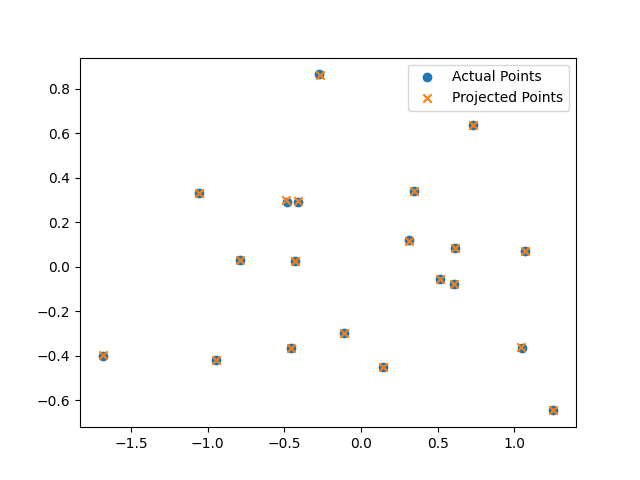
\includegraphics[width=10cm]{images/part1/normalize_1.png}
    \caption{Actual vs projected points}
\end{figure}

\begin{figure}[H]
    \centering
    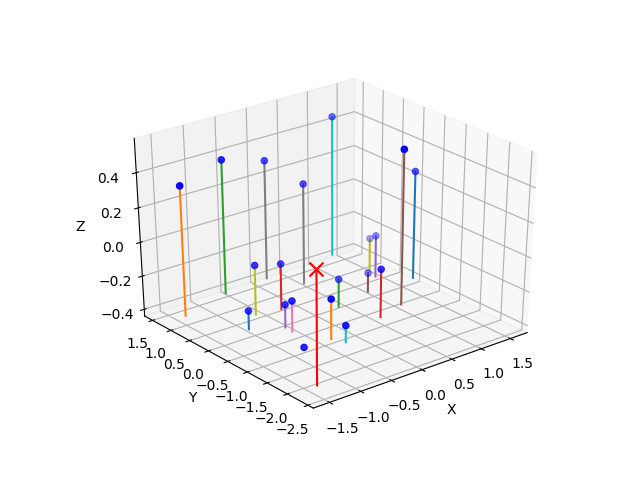
\includegraphics[width=10cm]{images/part1/normalize_2.png}
    \caption{Mô hình về camera's center và các điểm quan trọng trong thế giới thực '+' shows the camera centre, 'o' are the interest points}
\end{figure}

\textbf{Non-Normalized image coordinates (hard\_points=True)}

The projection matrix is:
\begin{equation*}
    \begin{bmatrix}
        -2.04662532e+00 &  1.18743052e+00 & 3.88938200e-01 & 2.43732985e+02    \\
        -4.56886722e-01 & -3.02017128e-01 & 2.14721848e+00 & 1.65932475e+02    \\
        -2.24678720e-03 & -1.09380146e-03 & 5.58547111e-04 & 1.00000000e+00
    \end{bmatrix}
\end{equation*}

The total residual is:

$15.621732302525796$

The estimated location of the camera is:
\begin{equation*}
    \begin{bmatrix}
        303.09666406 & 307.18423708 & 30.4222733
    \end{bmatrix}
\end{equation*}

\begin{figure}[H]
    \centering
    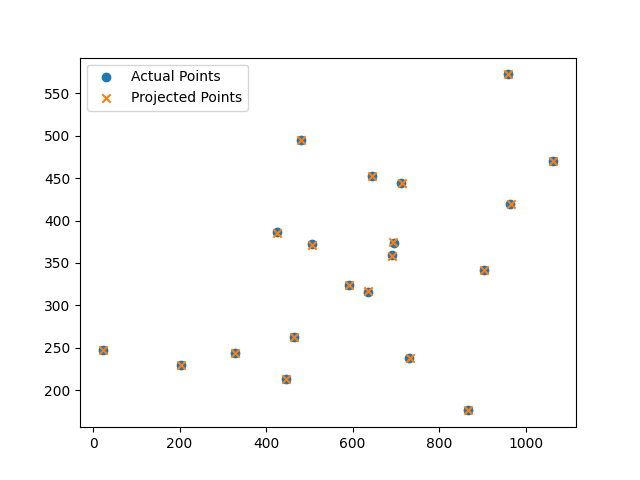
\includegraphics[width=10cm]{images/part1/non-normalize_1.png}
    \caption{Actual vs projected points}
\end{figure}

\begin{figure}[H]
    \centering
    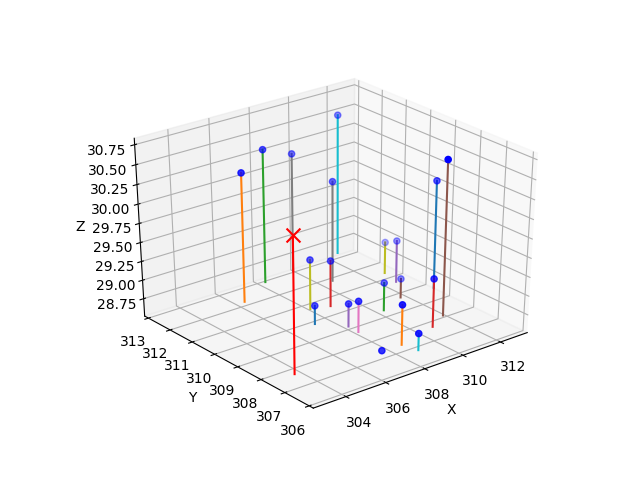
\includegraphics[width=10cm]{images/part1/non-normalize_2.png}
    \caption{Mô hình về camera's center và các điểm quan trọng trong thế giới thực '+' shows the camera centre, 'o' are the interest points}
\end{figure}

\section*{Estimation of Fundamental Matrix}
\subsection*{Chi tiết hiện thực}

Giải thuật 8-point được sử dụng để tính toán ma trận fundamental matrix (F) khi có các cặp điểm tương ứng với 2 ảnh. Với mỗi cặp điểm $x=(u, v)$ trong ảnh bên trái và $x'= (u',v')$ trong ảnh bên phải, ta có:
\begin{equation*}
    x'^T F x = 0
\end{equation*}
với n cặp điểm ta có:
\begin{align*}
    \begin{bmatrix}
        u'_1u_1 & u'_1v_1 & u'_1 & v'_1u_1 & v'_1v_1 & v'_1 & u_1 & v_1 & 1 \\
        \vdots & \vdots & \vdots & \vdots & \vdots & \vdots & \vdots & \vdots & \vdots \\
        u'_nu_n & u'_nv_n & u'_n & v'_nu_n & v'_nv_n & v'_n & u_n & v_n & 1
    \end{bmatrix}
    \begin{bmatrix}
        f_{11} \\
        f_{12} \\
        f_{13} \\
        f_{21} \\
        f_{22} \\
        f_{23} \\
        f_{31} \\
        f_{32} \\
        f_{33}
    \end{bmatrix}
    = 0
\end{align*}
giải ma trận F bằng cách sử dụng SVD:

Chi tiết hiện thực trong python/numpy:
\inputpython{code/part2_1.py}{1}{16}

\textbf{Normalized image coordinates}
\begin{equation*}
    \begin{bmatrix}
        u' \\
        v' \\
        1
    \end{bmatrix}
    =
    \begin{bmatrix}
        s & 0 & 0 \\
        0 & s & 0 \\
        0 & 0 & 1
    \end{bmatrix}
    \begin{bmatrix}
        1 & 0 & -\bar{u} \\
        0 & 1 & -\bar{v} \\
        0 & 0 & 1
    \end{bmatrix}
    \begin{bmatrix}
        u \\
        v \\
        1
    \end{bmatrix}
\end{equation*}

trong đó:
\begin{itemize}
    \item $(u', v', 1)$ là toạ độ đã được chuẩn hoá.
    \item $(u, v, 1)$ là toạ độ chưa được chuẩn hoá.
    \item $s$ là hệ số sacle.
    \item $\bar{u}, \bar{v}$ là giá trị trung bình trên tất cả các điểm.
\end{itemize}

Các bước thực hiện:
\begin{itemize}
    \item Tính toán trọng tâm của tất cả các điểm tương ứng với hai ảnh.
        \begin{equation*}
            \bar{u} = \dfrac{1}{n} \displaystyle \sum_{i=1}^{n} u_i
        \end{equation*}
        \begin{equation*}
            \bar{v} = \dfrac{1}{n} \displaystyle \sum_{i=1}^{n} v_i
        \end{equation*}
    \item Trừ toạ độ các điểm với mean.
        \begin{equation*}
            \tilde{u} = u - \bar{u}
        \end{equation*}
        \begin{equation*}
            \tilde{v} = v - \bar{v}
        \end{equation*}
    \item  Tính toán hệ số sacle s dựa theo công thức:
        \begin{equation*}
            s = \dfrac{\sqrt{2}}{\sqrt{(\dfrac{1}{n}\displaystyle \sum_{i=1}^{n} (\tilde{u}_i^2 + \tilde{v}_i^2))}}
        \end{equation*}
        \begin{equation*}
            s' = \dfrac{\sqrt{2}}{\sqrt{(\dfrac{1}{n}\displaystyle \sum_{i=1}^{n} (\tilde{u'}_i^2 + \tilde{v'}_i^2))}}
        \end{equation*}
    \item Xây dựng ma trận $T_a, T_b$:
        \begin{equation*}
            T_a = 
            \begin{bmatrix}
                s & 0 & 0 \\
                0 & s & 0 \\
                0 & 0 & 1
            \end{bmatrix}
            \begin{bmatrix}
                1 & 0 & -\bar{u} \\
                0 & 1 & -\bar{v} \\
                0 & 0 & 1
            \end{bmatrix}
        \end{equation*}
        \begin{equation*}
            T_b = 
            \begin{bmatrix}
                s' & 0 & 0 \\
                0 & s' & 0 \\
                0 & 0 & 1
            \end{bmatrix}
            \begin{bmatrix}
                1 & 0 & -\bar{u'} \\
                0 & 1 & -\bar{v'} \\
                0 & 0 & 1
            \end{bmatrix}
        \end{equation*}
    \item Tính toạ độ sau khi chuẩn hoá:
        \begin{equation*}
            \hat{x}_i = T_a x
        \end{equation*}
        \begin{equation*}
            \hat{x'}_i = T_b x'
        \end{equation*}
    \item Tính ma trận Fundamental Matrix dựa vào toạ độ sau khi chuẩn hoá tương tự như giải thuật 8-point ở trên.
    \item Sau khi tính được ma trận $F_{\mathit{norm}}$, ma trận $F_{\mathit{orig}}$ được tính dựa theo công thức sau:
        \begin{equation*}
            F_{\mathit{orig}} = T_b^T \ast F_{norm} \ast T_{a}
        \end{equation*}
\end{itemize}

Chi tiết hiện thực trong python/numpy:
\inputpython{code/part2_2.py}{1}{38}


\subsection*{Kết quả}
\textbf{Normalized image coordinates}

Fundamental Matrix:
\begin{equation*}
    \begin{bmatrix}
        -1.17248591e-07 & 1.60824663e-06 &-4.01980786e-04    \\
        1.11212887e-06 &-2.73443755e-07 & 3.23319884e-03    \\
        -2.36400817e-05 & -4.44404958e-03 & 1.03455561e-01
    \end{bmatrix}
\end{equation*}

\begin{figure}[H]
    \centering
    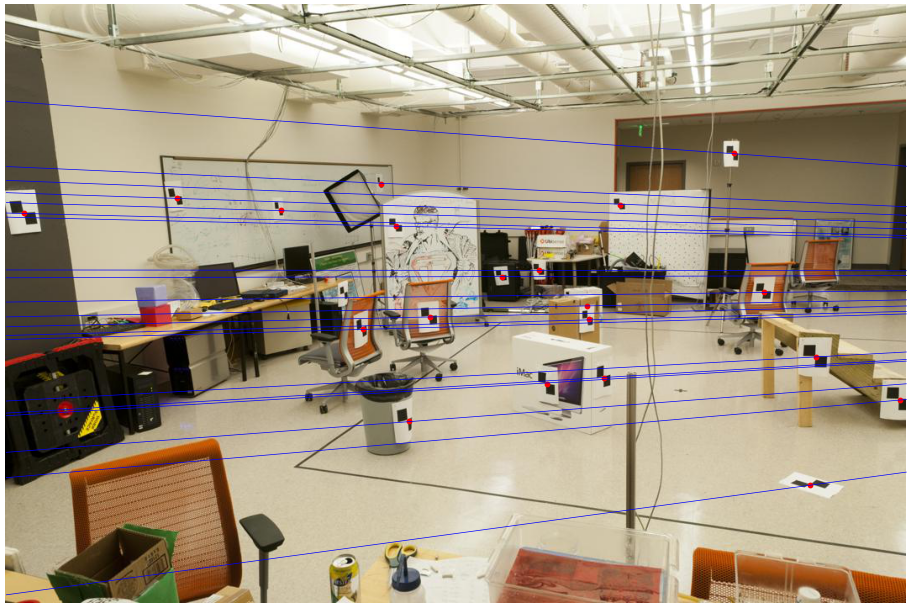
\includegraphics[width=15cm]{images/part2/normalize_1_left.png}
    \caption{Left image, Normalized image coordinates}
\end{figure}

\begin{figure}[H]
    \centering
    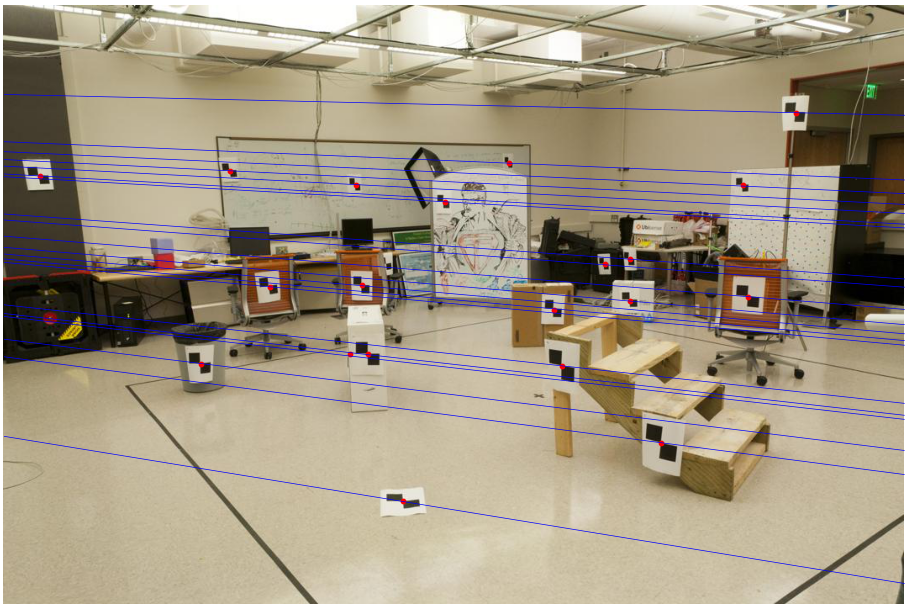
\includegraphics[width=15cm]{images/part2/normalize_1_right.png}
    \caption{Right image, Normalized image coordinates}
\end{figure}

\begin{figure}[H]
    \centering
    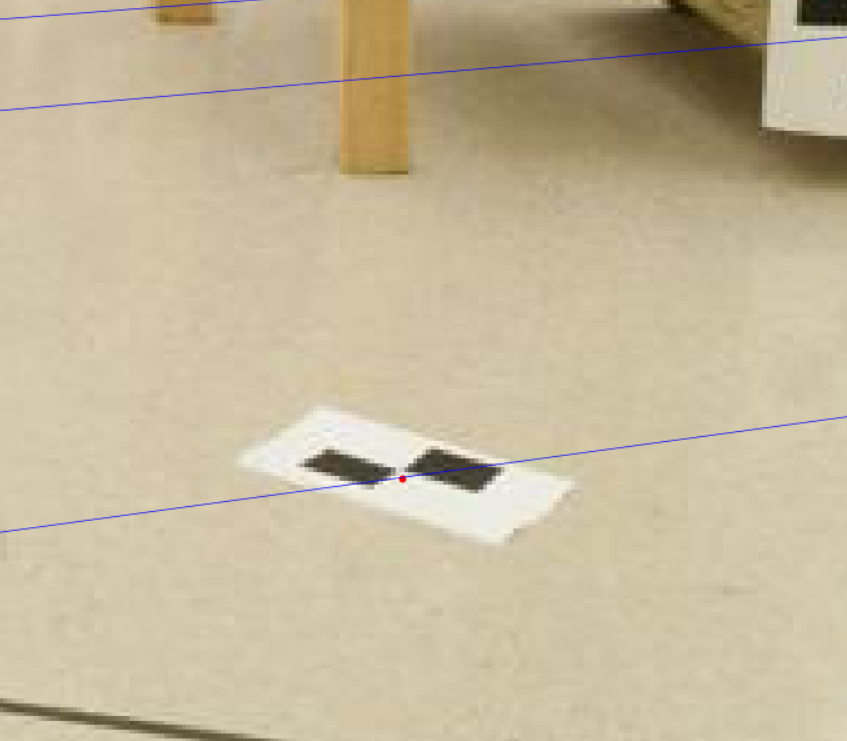
\includegraphics[width=6cm]{images/part2/normalize_1_left_zoom.png}
    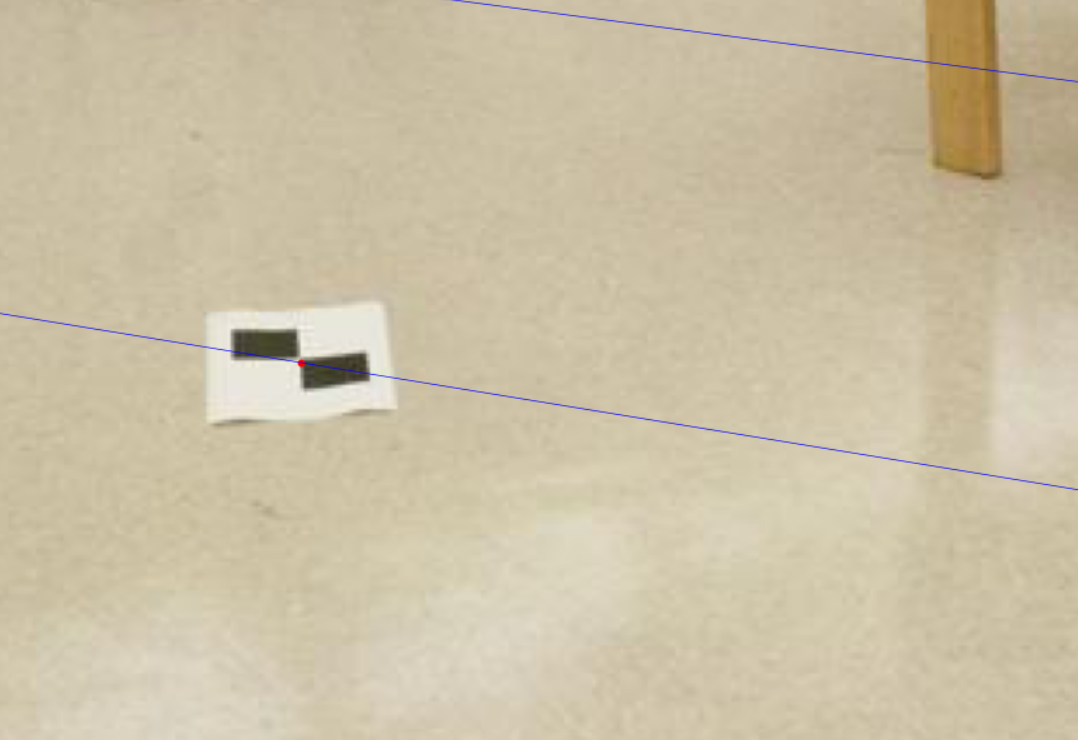
\includegraphics[width=6cm]{images/part2/normalize_1_right_zoom.png}
    \caption{\emph{Left:} Left zoom, \emph{Right:} Right zoom}
\end{figure}

\textbf{Non-Normalized image coordinates}

Fundamental Matrix:
\begin{equation*}
    \begin{bmatrix}
        -5.36264198e-07 & 7.90364771e-06 & -1.88600204e-03  \\
        8.83539184e-06 & 1.21321685e-06 & 1.72332901e-02    \\
        -9.07382264e-04 & -2.64234650e-02 & 9.99500092e-01
    \end{bmatrix}
\end{equation*}

\begin{figure}[H]
    \centering
    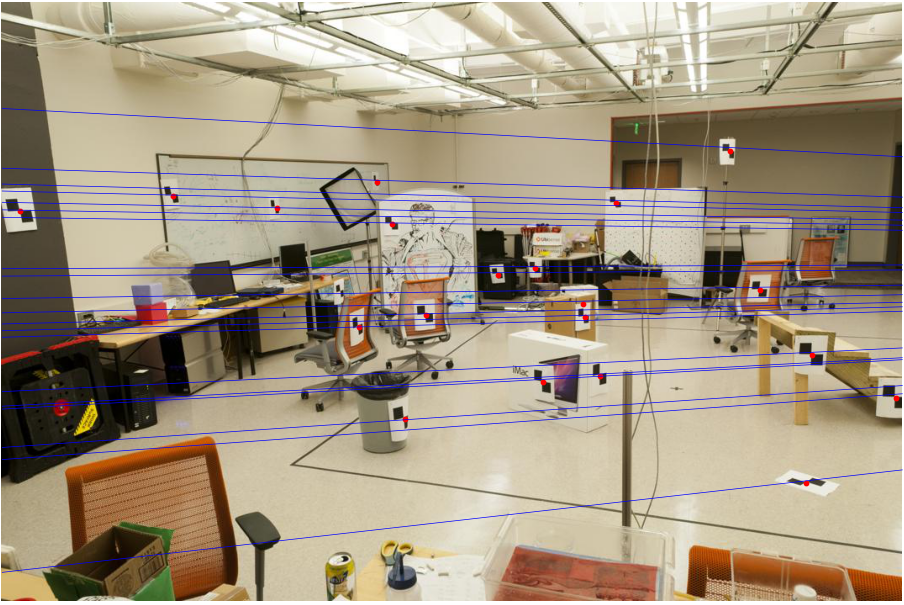
\includegraphics[width=15cm]{images/part2/non-normalize_1_left.png}
    \caption{Left image, Non-normalized image coordinates}
\end{figure}

\begin{figure}[H]
    \centering
    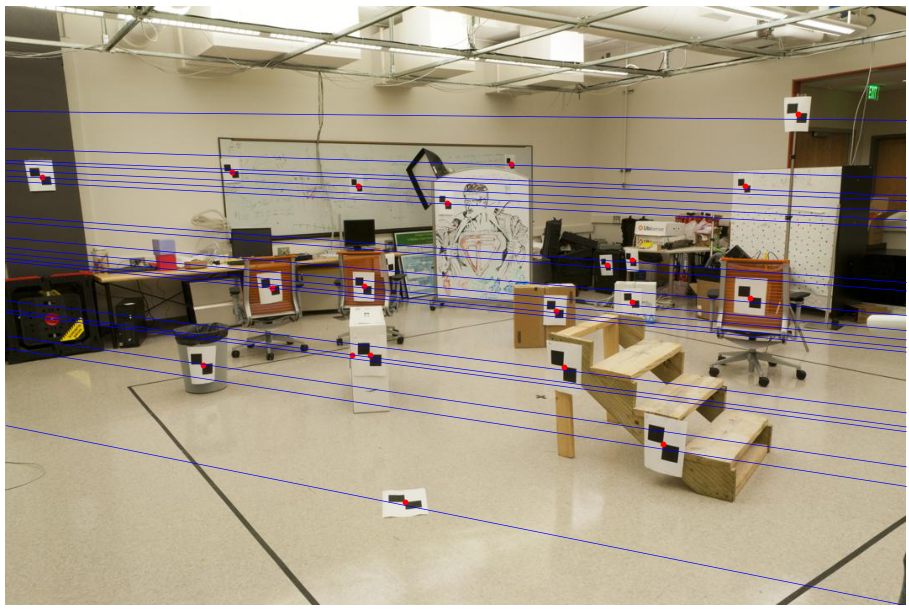
\includegraphics[width=15cm]{images/part2/non-normalize_1_right.png}
    \caption{Right image, Non-normalized image coordinates}
\end{figure}

\begin{figure}[H]
    \centering
    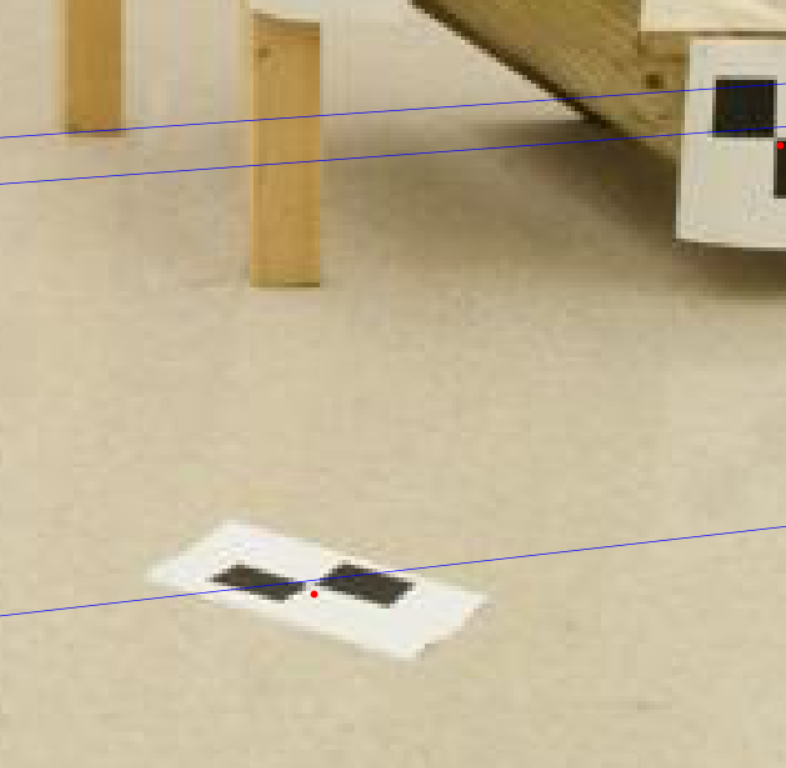
\includegraphics[width=6cm]{images/part2/non-normalize_1_left_zoom.png}
    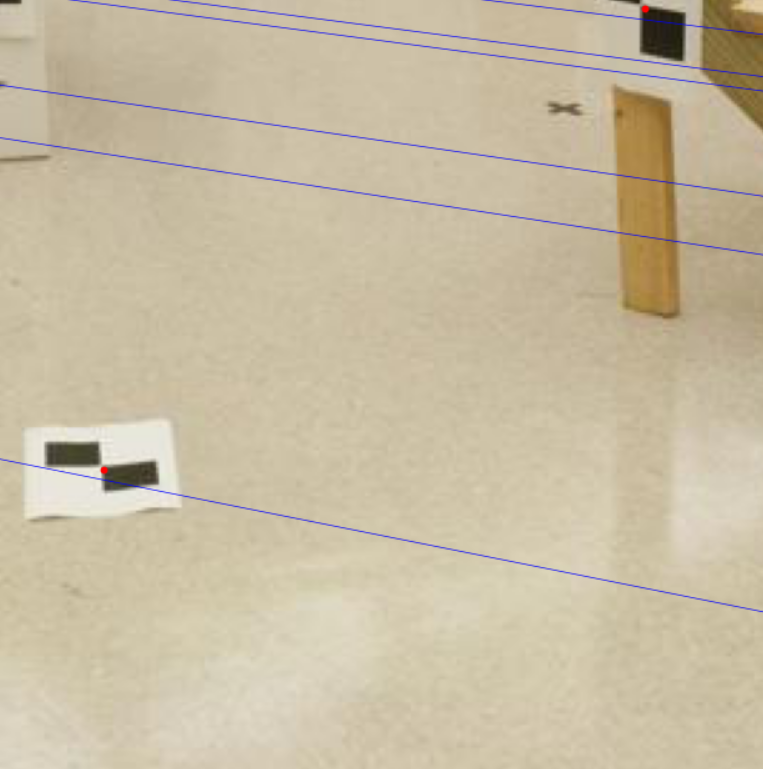
\includegraphics[width=6cm]{images/part2/non-normalize_1_right_zoom.png}
    \caption{\emph{Left:} Left zoom, \emph{Right:} Right zoom}
\end{figure}

\section*{Fundamental Matrix with RANSAC}
\subsection*{Chi tiết hiện thực}
Các bước thực hiện giải thuật RANSAC:
\begin{itemize}
    \item Chọn ngầu nhiên 8 cặp điểm giữa 2 ảnh.
    \item Tính toán ma trận Fundamental dựa trên các cặp điểm đã chọn.
    \item Từ ma trận F đã tính được, tính tổng số inlier dựa theo công thức:
        \begin{equation*}
            \text{if} \; (x'^T F x \leq \text{threshold}) \Rightarrow \text{inlier}
        \end{equation*}
    \item Lặp lại giải thuật một số lần lặp nhất định.
    \item Chọn ma trận Fundamental cho số inlier lớn nhất.
\end{itemize}

Chi tiết hiện thực trong python/numpy:
\inputpython{code/part3_1.py}{1}{27}

\subsection*{Kết quả}
\textbf{Sử dụng RANSAC}

\textbf{mt\_rushmore}


Noise ratio = 0.0
\begin{figure}[H]
    \centering
    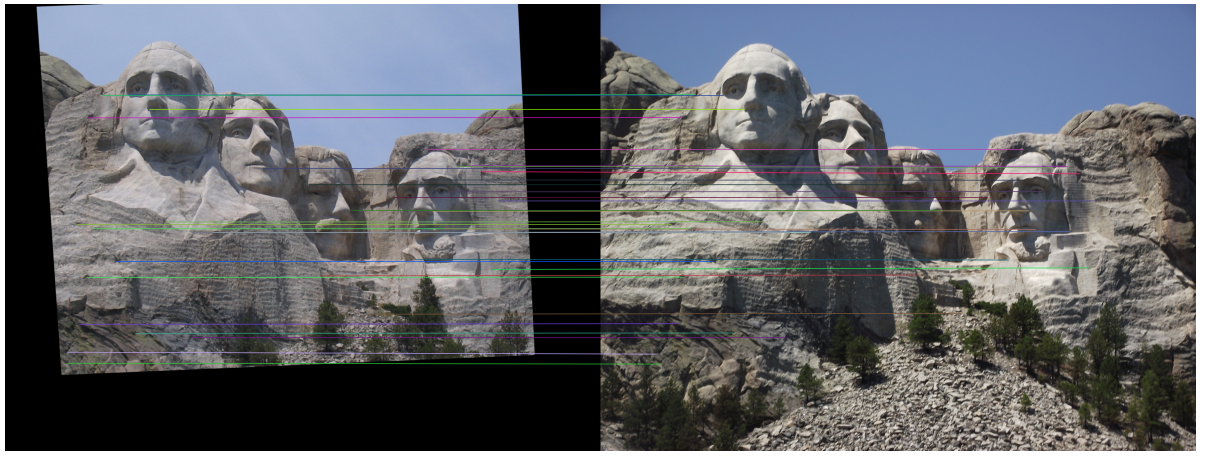
\includegraphics[width=14cm]{images/part3/ransac_image_1_noise_0.0_1.png}
\end{figure}

\begin{figure}[H]
    \centering
    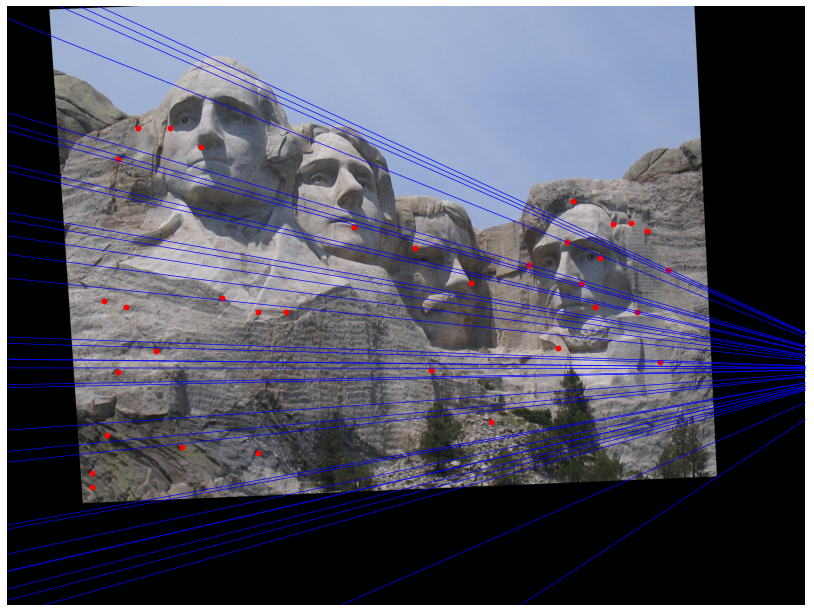
\includegraphics[width=6.5cm]{images/part3/ransac_image_1_noise_0.0_left.png}
    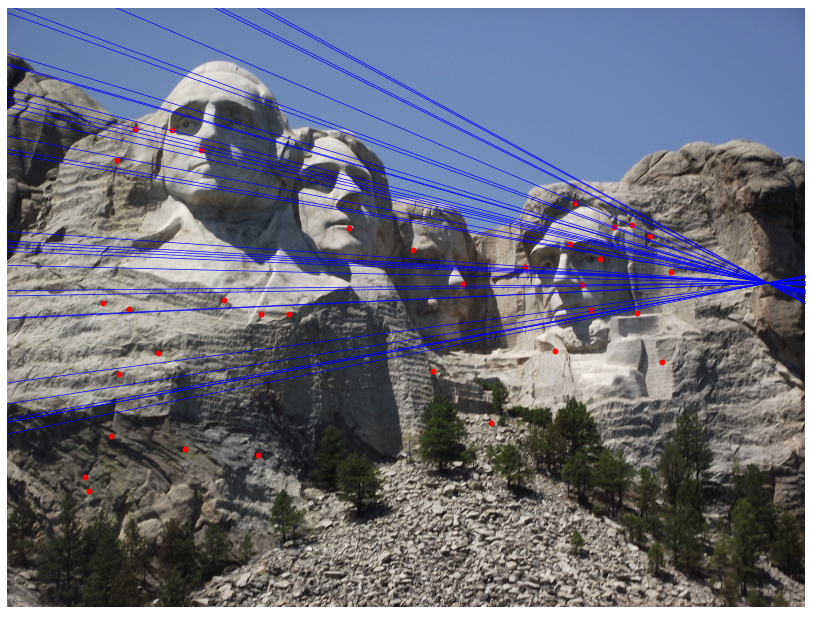
\includegraphics[width=6.5cm]{images/part3/ransac_image_1_noise_0.0_right.png}
\end{figure}

Noise ratio = 0.1
\begin{figure}[H]
    \centering
    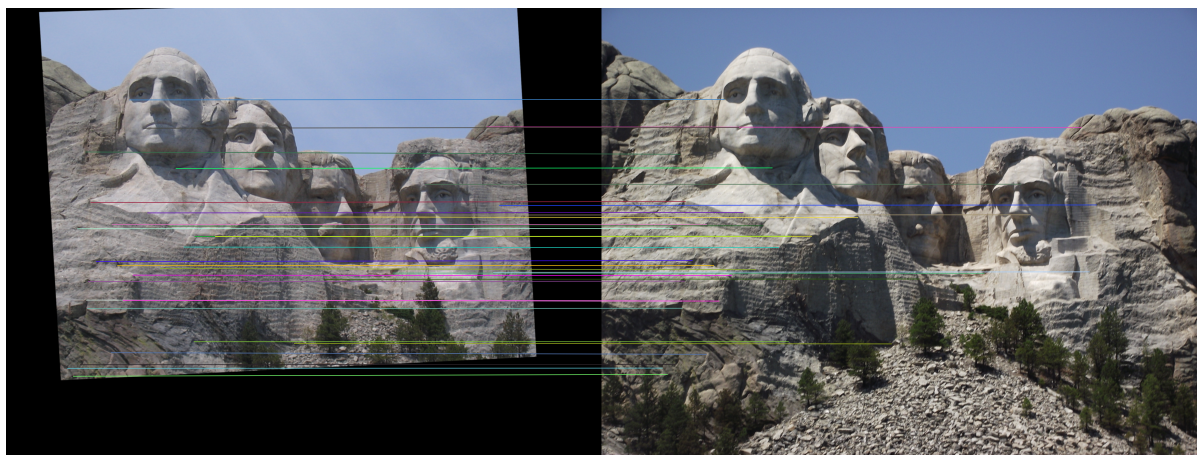
\includegraphics[width=14cm]{images/part3/ransac_image_1_noise_0.1_1.png}
\end{figure}

\begin{figure}[H]
    \centering
    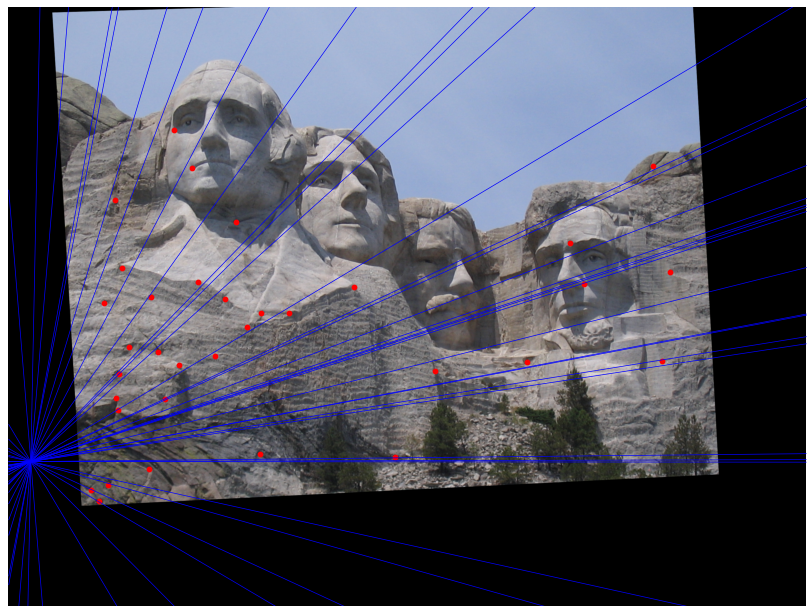
\includegraphics[width=6.5cm]{images/part3/ransac_image_1_noise_0.1_left.png}
    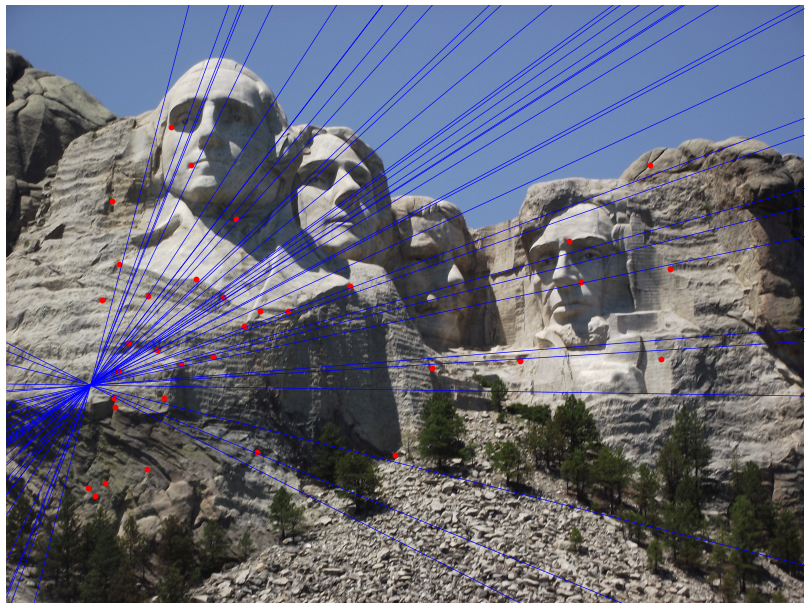
\includegraphics[width=6.5cm]{images/part3/ransac_image_1_noise_0.1_right.png}
\end{figure}

Noise ratio = 0.2
\begin{figure}[H]
    \centering
    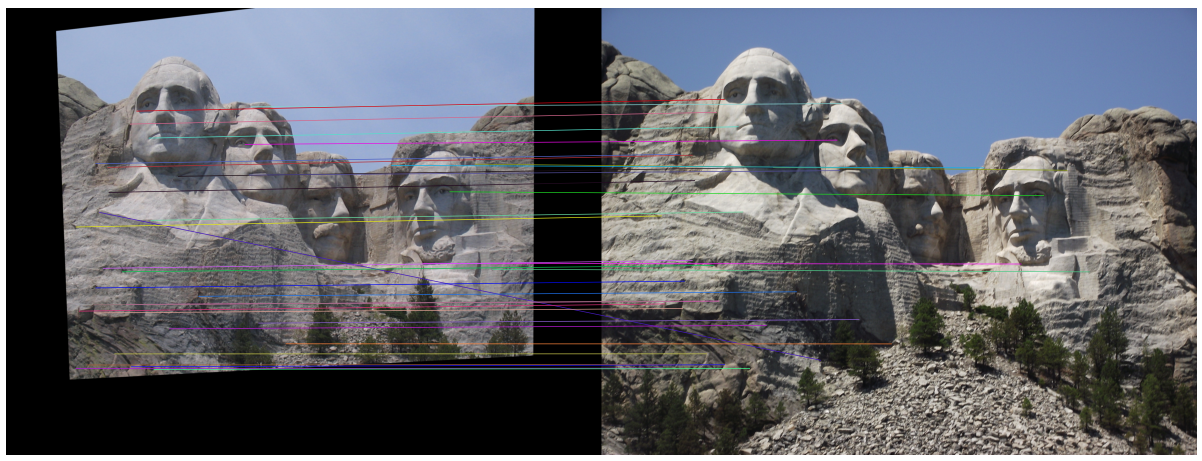
\includegraphics[width=14cm]{images/part3/ransac_image_1_noise_0.2_1.png}
\end{figure}

\begin{figure}[H]
    \centering
    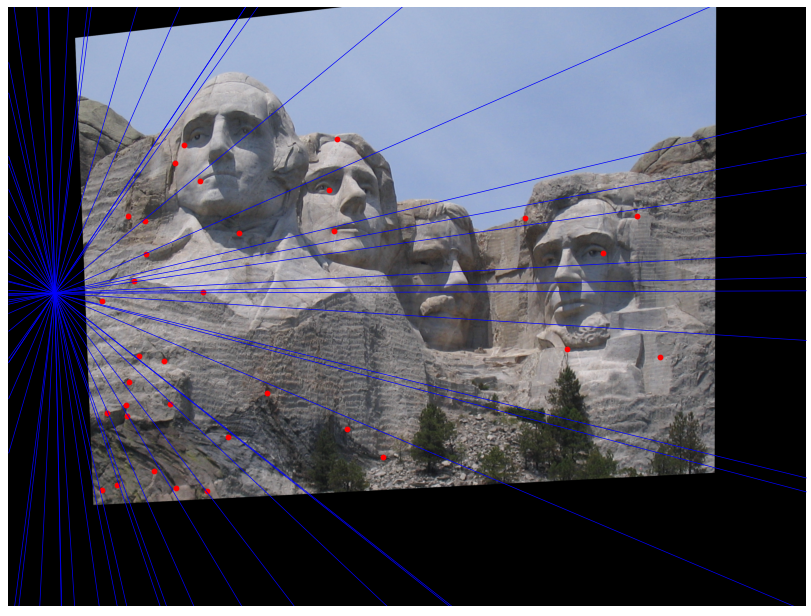
\includegraphics[width=6.5cm]{images/part3/ransac_image_1_noise_0.2_left.png}
    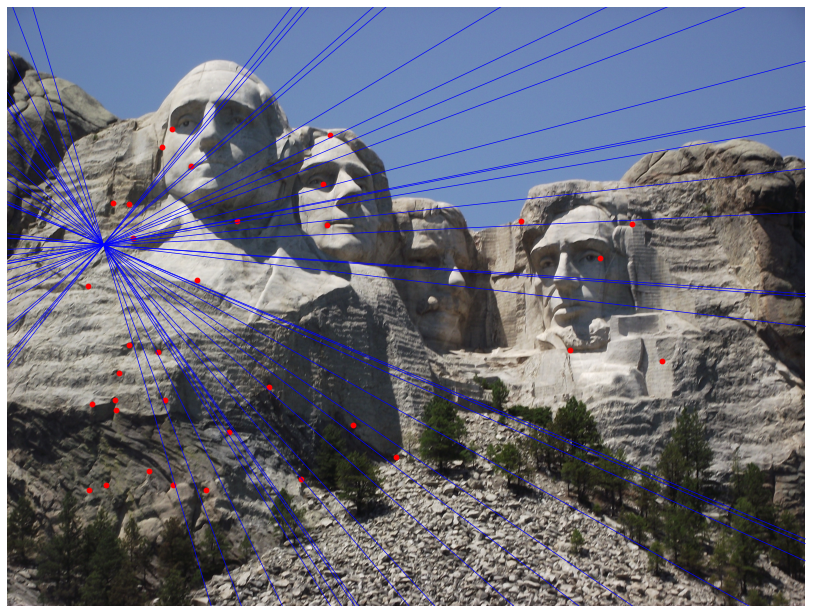
\includegraphics[width=6.5cm]{images/part3/ransac_image_1_noise_0.2_right.png}
\end{figure}

Noise ratio = 0.3
\begin{figure}[H]
    \centering
    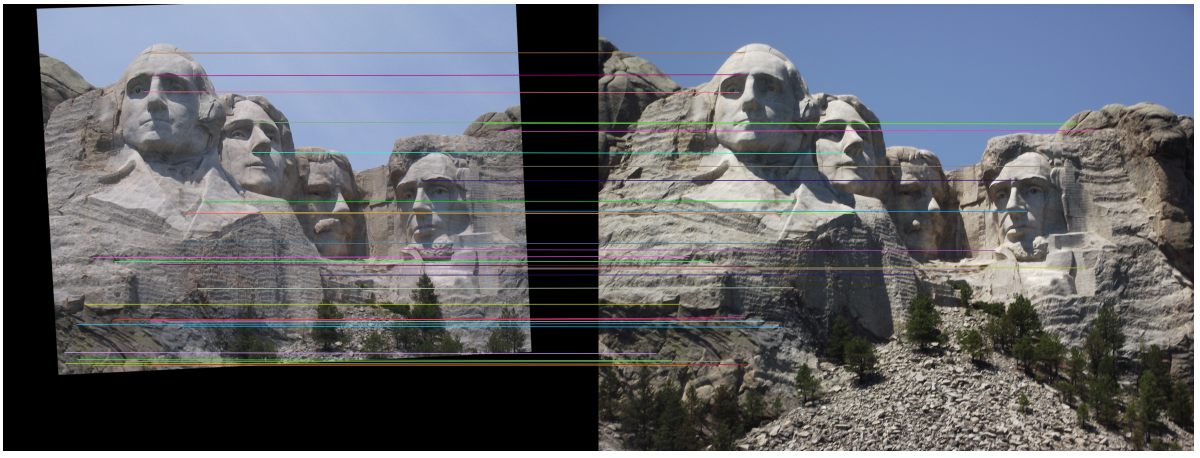
\includegraphics[width=14cm]{images/part3/ransac_image_1_noise_0.3_1.png}
\end{figure}

\begin{figure}[H]
    \centering
    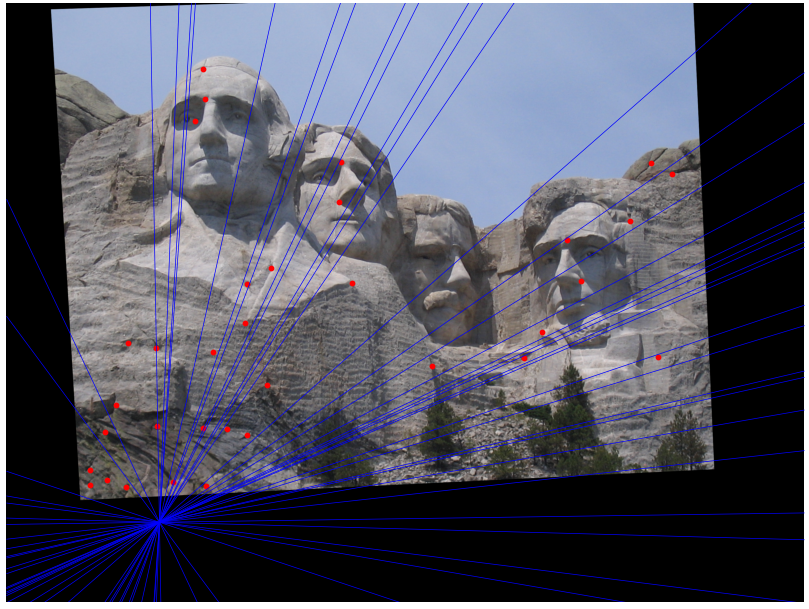
\includegraphics[width=6.5cm]{images/part3/ransac_image_1_noise_0.3_left.png}
    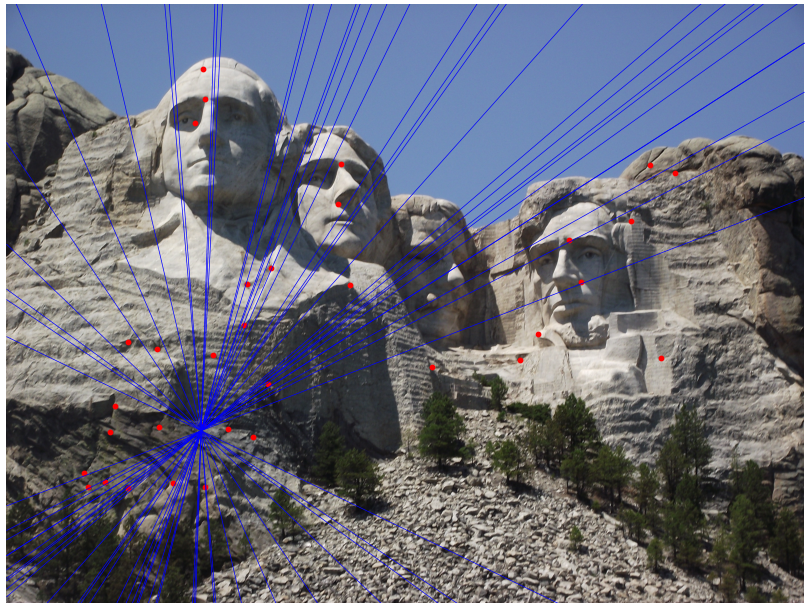
\includegraphics[width=6.5cm]{images/part3/ransac_image_1_noise_0.3_right.png}
\end{figure}

Noise ratio = 0.4
\begin{figure}[H]
    \centering
    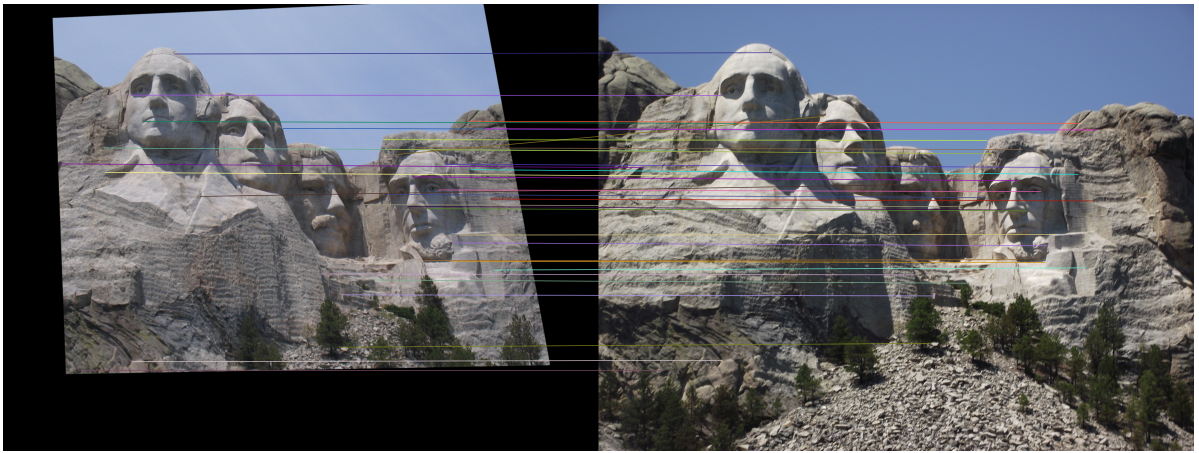
\includegraphics[width=14cm]{images/part3/ransac_image_1_noise_0.4_1.png}
\end{figure}

\begin{figure}[H]
    \centering
    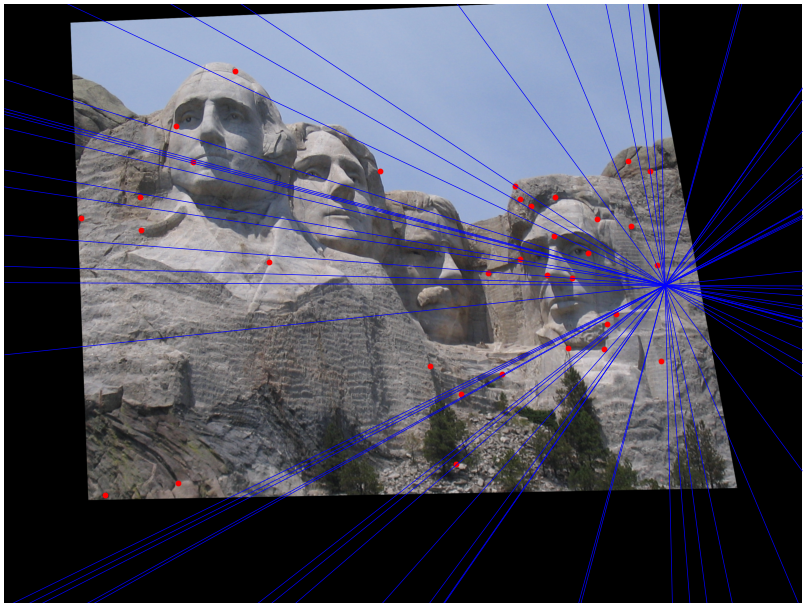
\includegraphics[width=6.5cm]{images/part3/ransac_image_1_noise_0.4_left.png}
    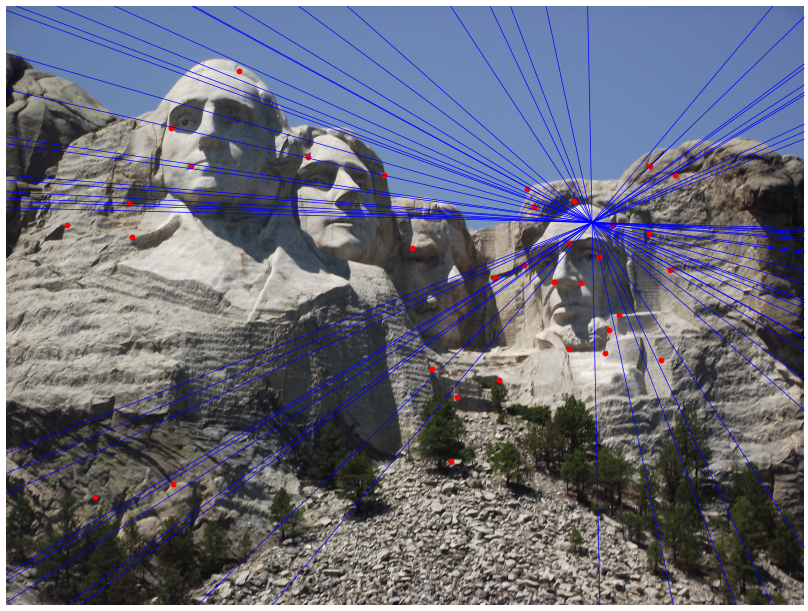
\includegraphics[width=6.5cm]{images/part3/ransac_image_1_noise_0.4_right.png}
\end{figure}

\textbf{notre\_dame}

Noise ratio = 0.2
\begin{figure}[H]
    \centering
    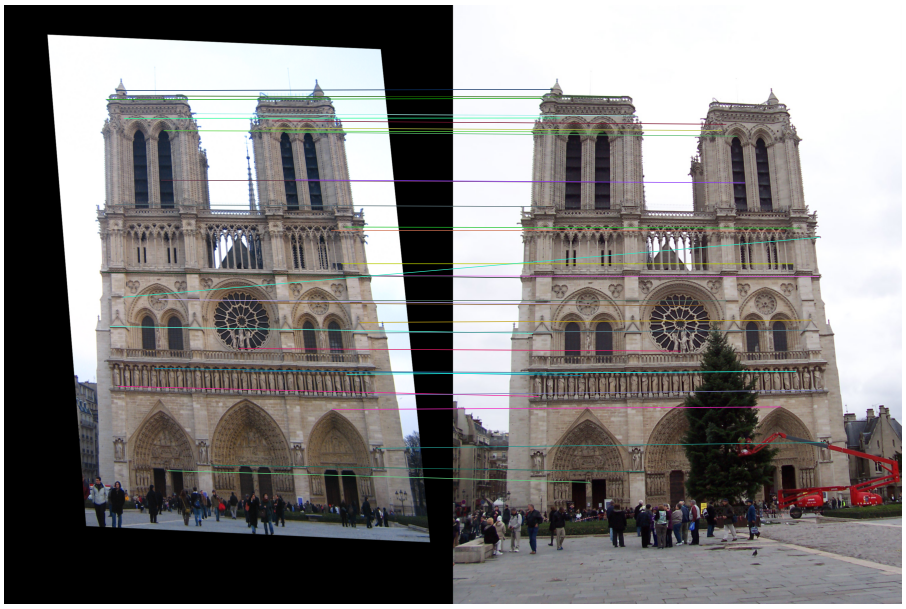
\includegraphics[width=10cm]{images/part3/ransac_image_2_noise_0.2_1.png}
\end{figure}

\begin{figure}[H]
    \centering
    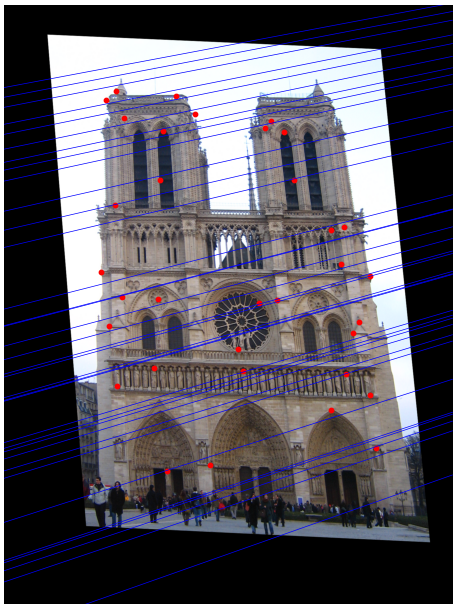
\includegraphics[width=4cm]{images/part3/ransac_image_2_noise_0.2_left.png}
    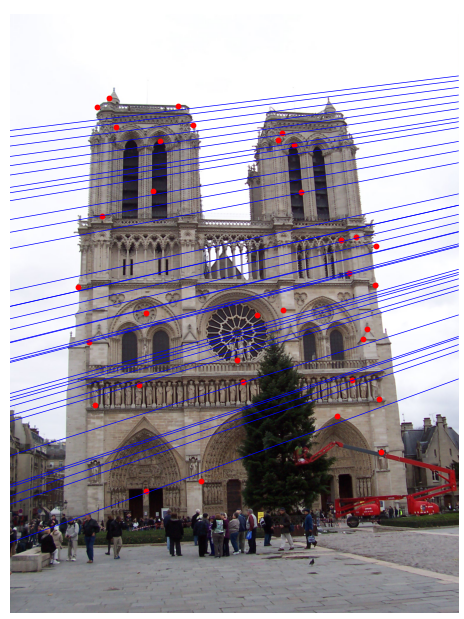
\includegraphics[width=4cm]{images/part3/ransac_image_2_noise_0.2_right.png}
\end{figure}

\textbf{gaudi}

Noise ratio = 0.2
\begin{figure}[H]
    \centering
    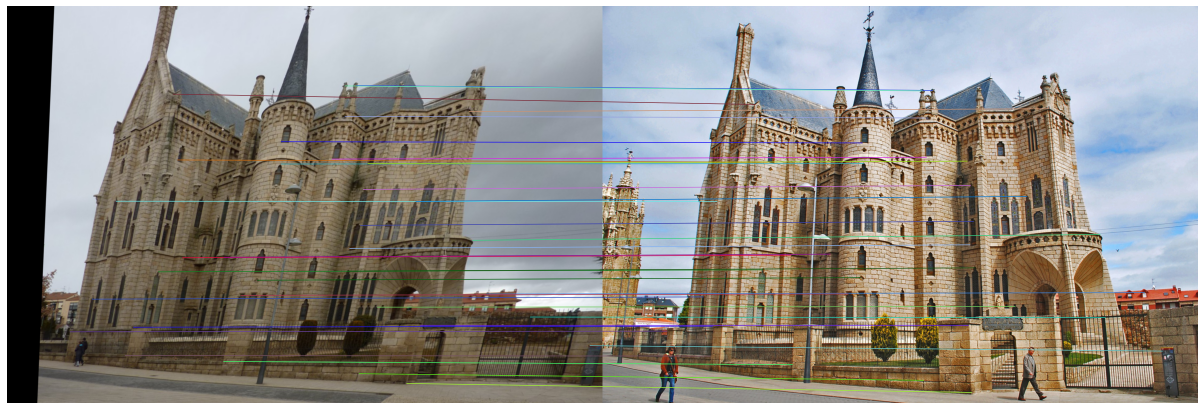
\includegraphics[width=14cm]{images/part3/ransac_image_3_noise_0.2_1.png}
\end{figure}

\begin{figure}[H]
    \centering
    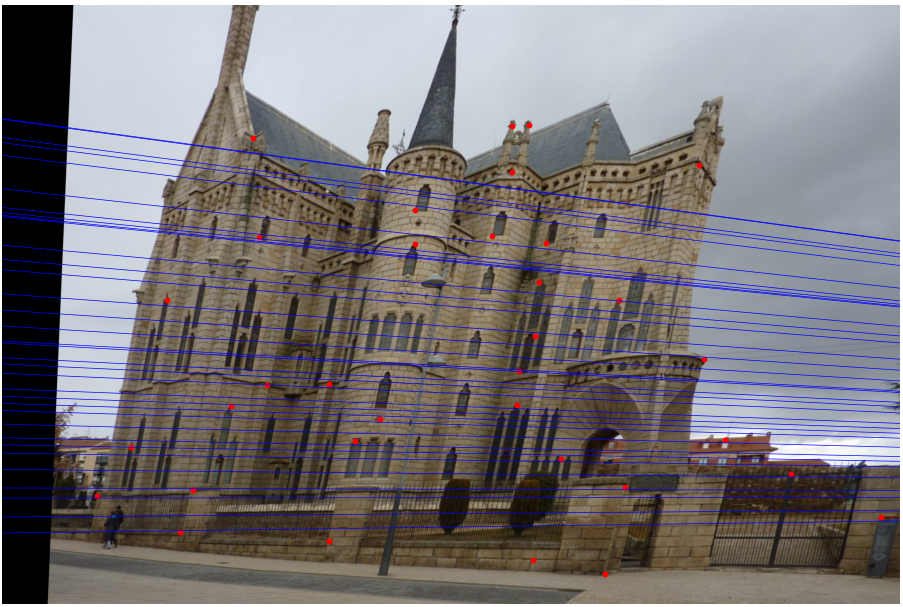
\includegraphics[width=6.5cm]{images/part3/ransac_image_3_noise_0.2_left.png}
    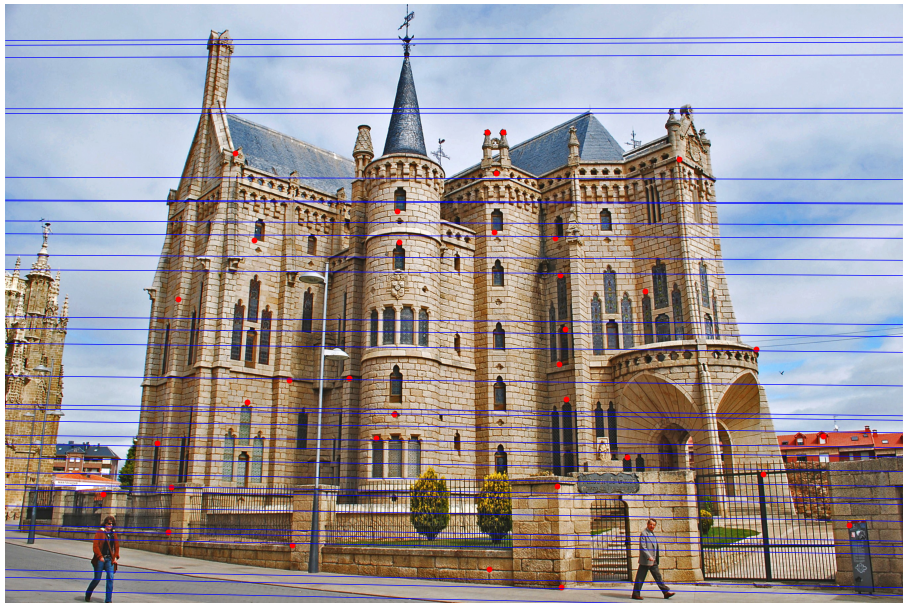
\includegraphics[width=6.5cm]{images/part3/ransac_image_3_noise_0.2_right.png}
\end{figure}

\textbf{Không sử dụng RANSAC}

Noise ratio = 0.1
\begin{figure}[H]
    \centering
    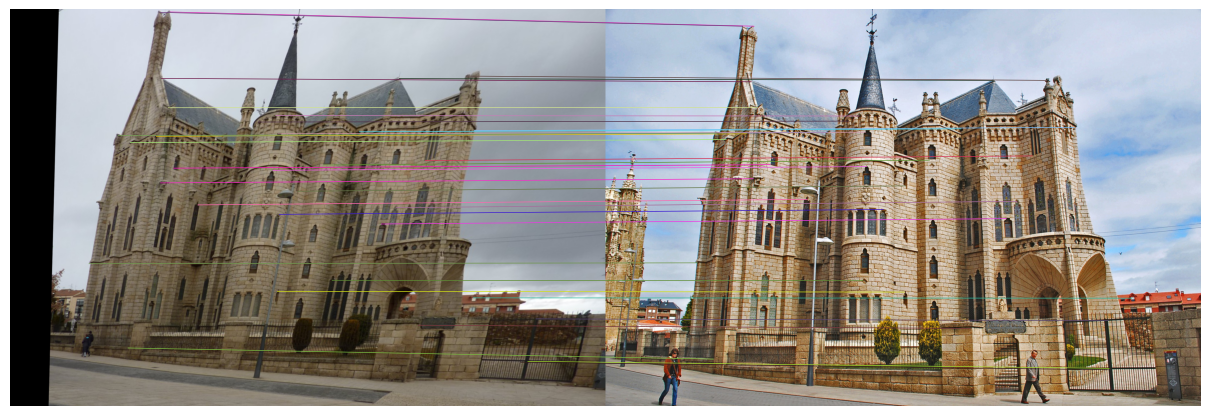
\includegraphics[width=14cm]{images/part3/no_ransac_image_1_noise_0.1_1.png}
\end{figure}

\begin{figure}[H]
    \centering
    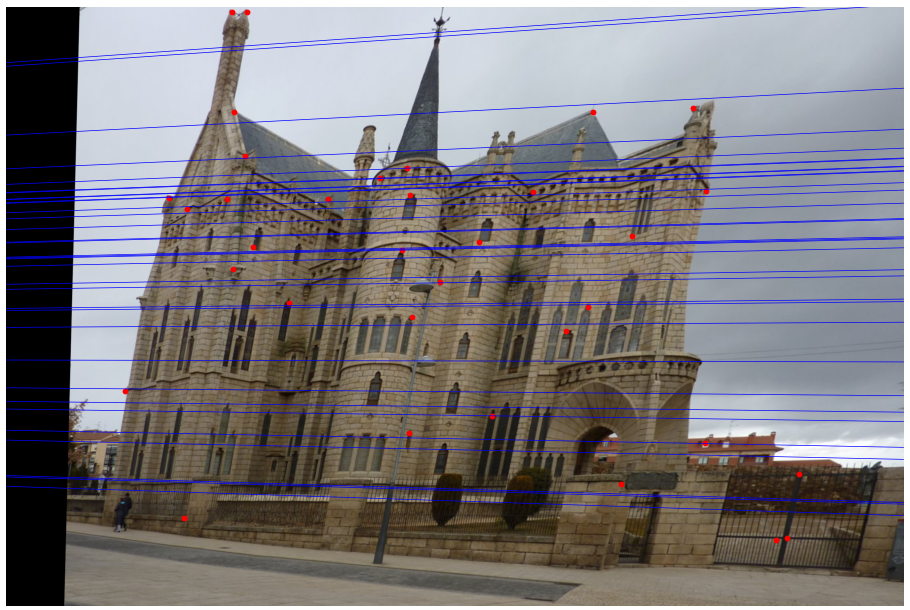
\includegraphics[width=6.5cm]{images/part3/no_ransac_image_1_noise_0.1_left.png}
    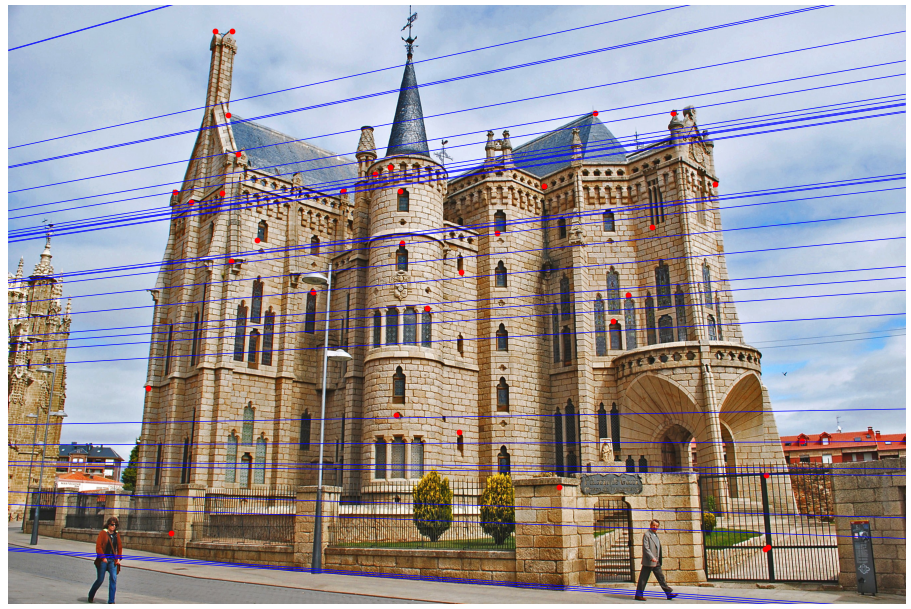
\includegraphics[width=6.5cm]{images/part3/no_ransac_image_1_noise_0.1_right.png}
\end{figure}

Noise ratio = 0.2
\begin{figure}[H]
    \centering
    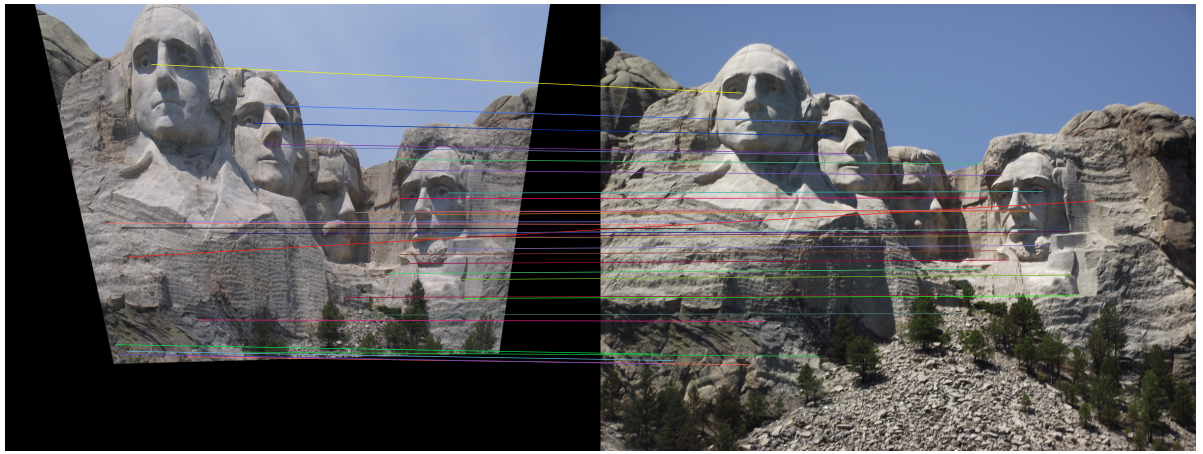
\includegraphics[width=14cm]{images/part3/no_ransac_image_1_noise_0.2_1.png}
\end{figure}

\begin{figure}[H]
    \centering
    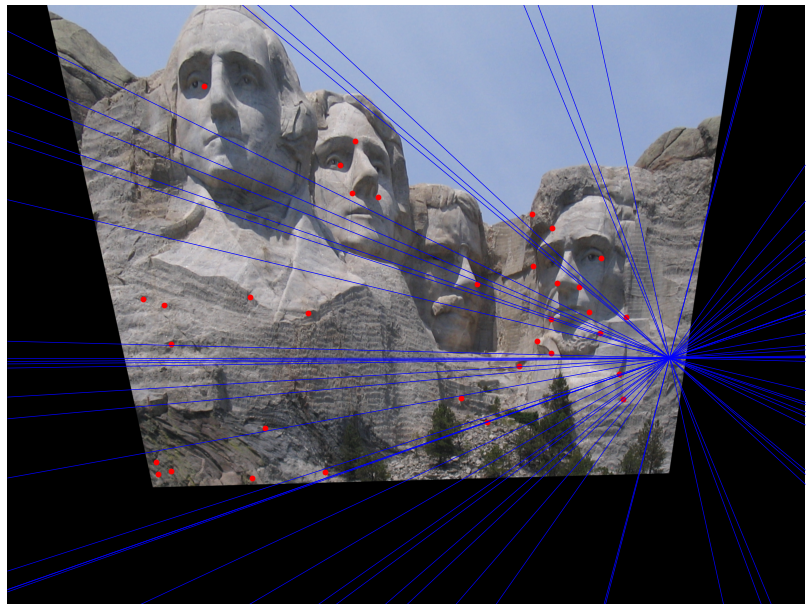
\includegraphics[width=6.5cm]{images/part3/no_ransac_image_1_noise_0.2_left.png}
    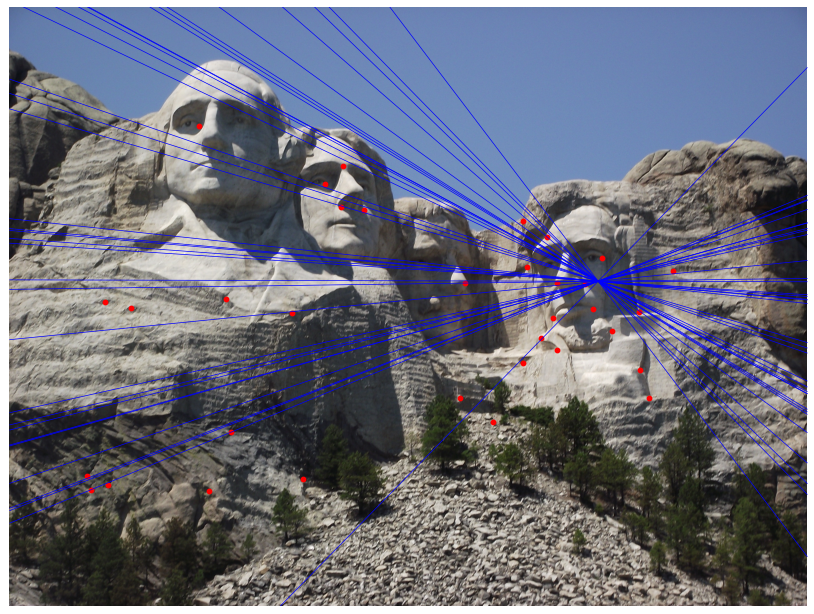
\includegraphics[width=6.5cm]{images/part3/no_ransac_image_1_noise_0.2_right.png}
\end{figure}

Noise ratio = 0.3
\begin{figure}[H]
    \centering
    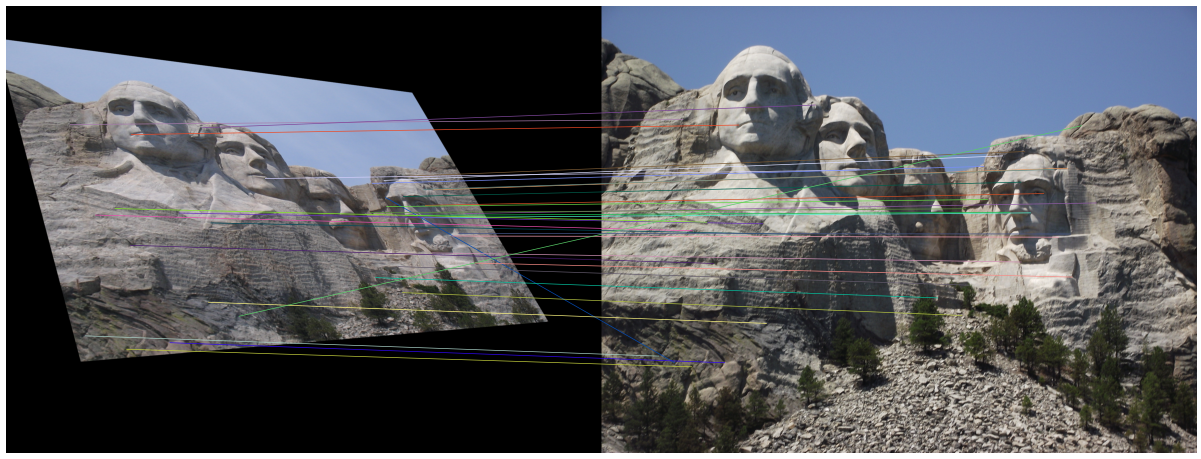
\includegraphics[width=14cm]{images/part3/no_ransac_image_1_noise_0.3_1.png}
\end{figure}

\begin{figure}[H]
    \centering
    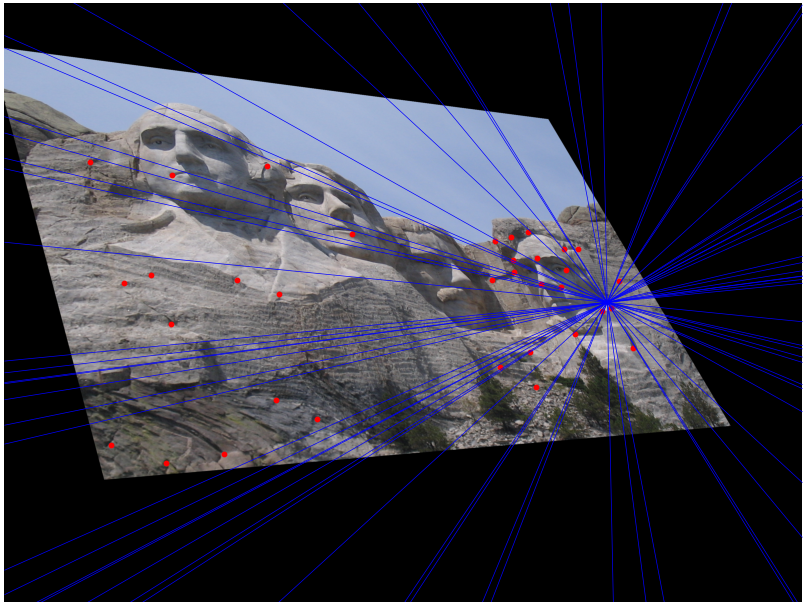
\includegraphics[width=6.5cm]{images/part3/no_ransac_image_1_noise_0.3_left.png}
    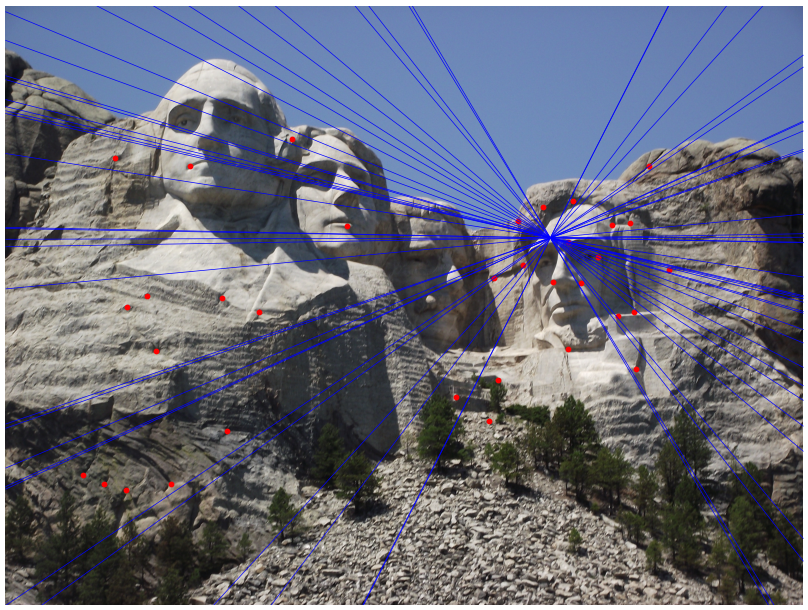
\includegraphics[width=6.5cm]{images/part3/no_ransac_image_1_noise_0.3_right.png}
\end{figure}

Noise ratio = 0.4
\begin{figure}[H]
    \centering
    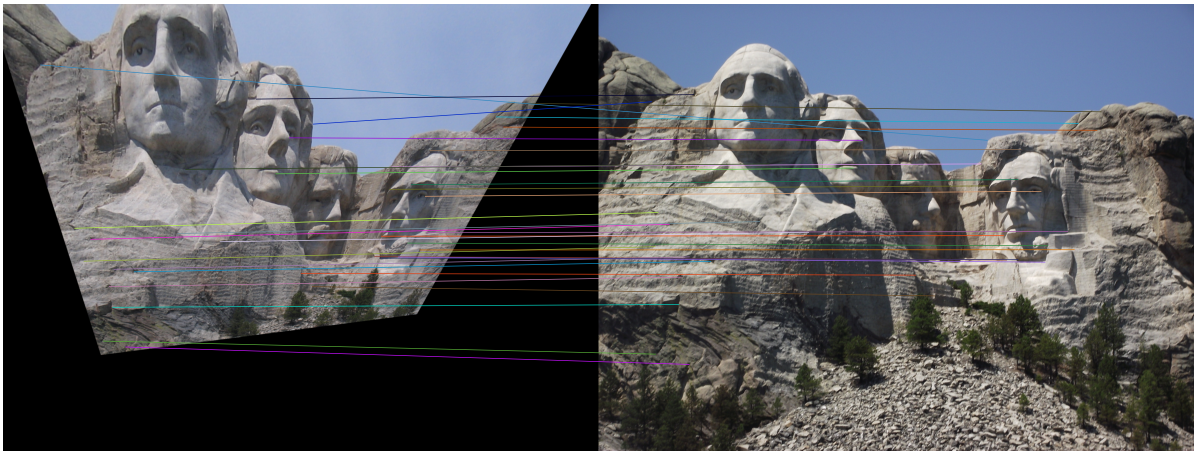
\includegraphics[width=14cm]{images/part3/no_ransac_image_1_noise_0.4_1.png}
\end{figure}

\begin{figure}[H]
    \centering
    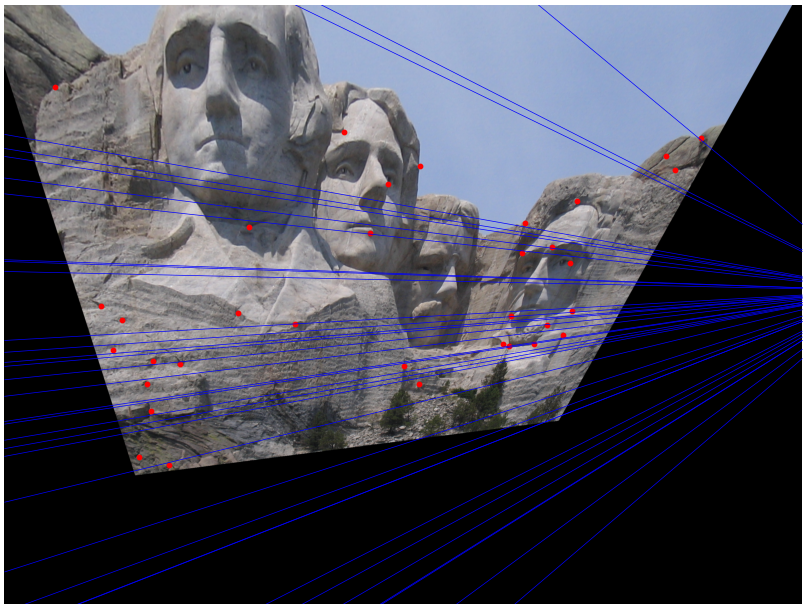
\includegraphics[width=6.5cm]{images/part3/no_ransac_image_1_noise_0.4_left.png}
    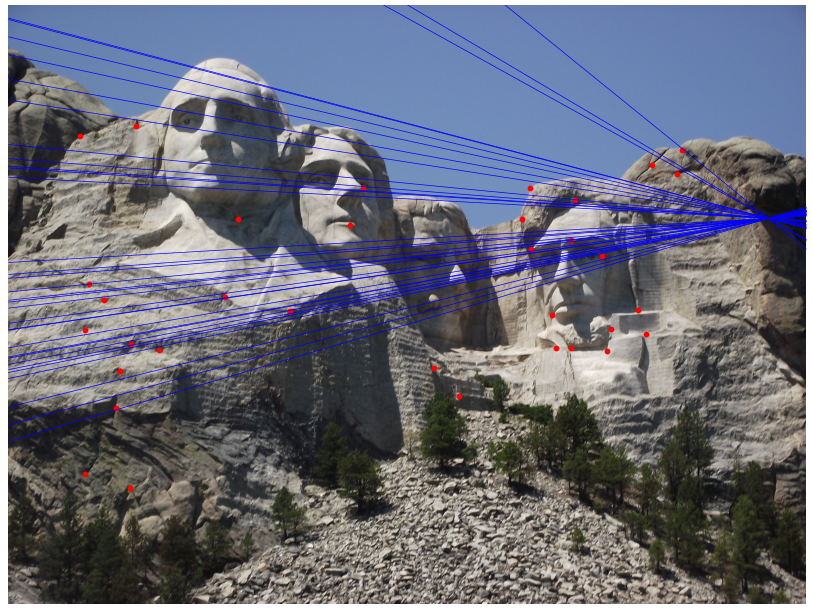
\includegraphics[width=6.5cm]{images/part3/no_ransac_image_1_noise_0.4_right.png}
\end{figure}


\textbf{Sử dụng ORB features}
mt\_rushmore:
\begin{figure}[H]
    \centering
    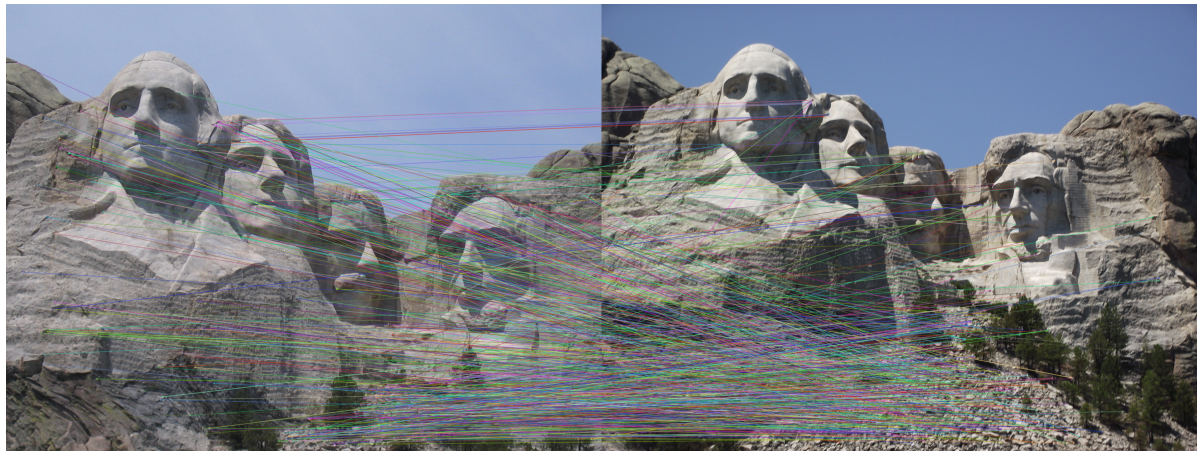
\includegraphics[width=14cm]{images/part3/orb_image_1_0.png}
\end{figure}
\begin{figure}[H]
    \centering
    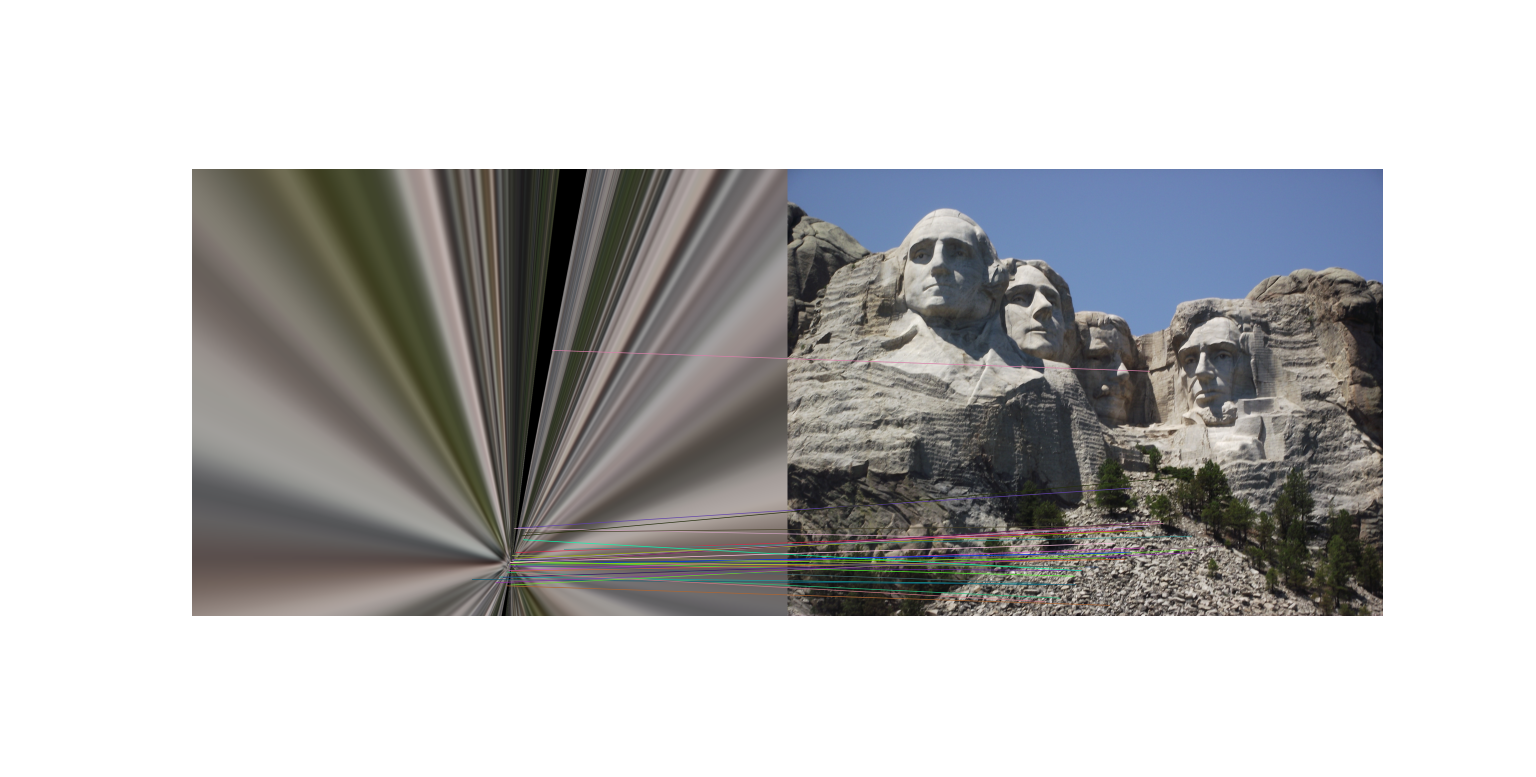
\includegraphics[width=14cm]{images/part3/orb_image_1_1.png}
\end{figure}

notre\_dame:
\begin{figure}[H]
    \centering
    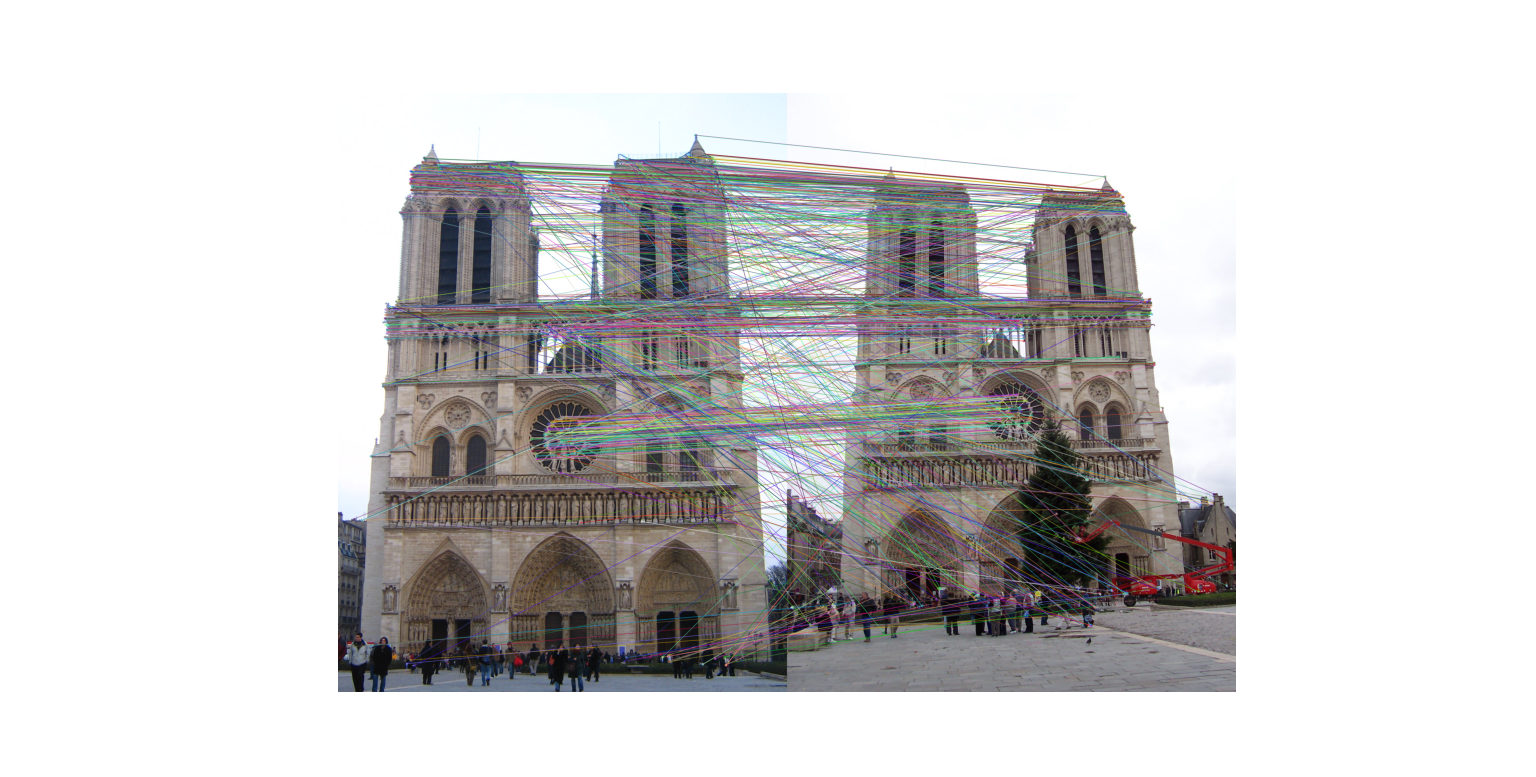
\includegraphics[width=14cm]{images/part3/orb_image_2_0.png}
\end{figure}
\begin{figure}[H]
    \centering
    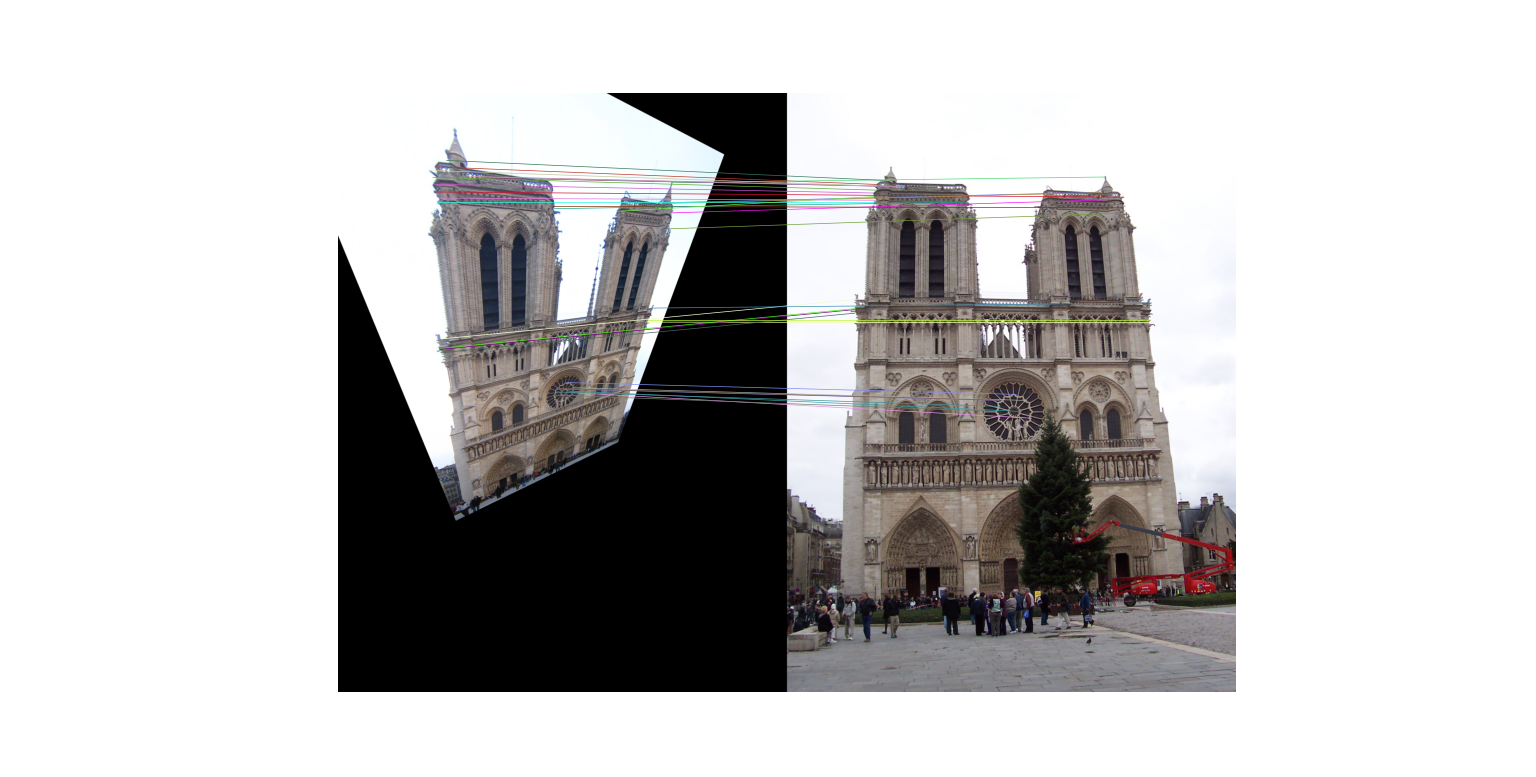
\includegraphics[width=14cm]{images/part3/orb_image_2_1.png}
\end{figure}

gaudi:
\begin{figure}[H]
    \centering
    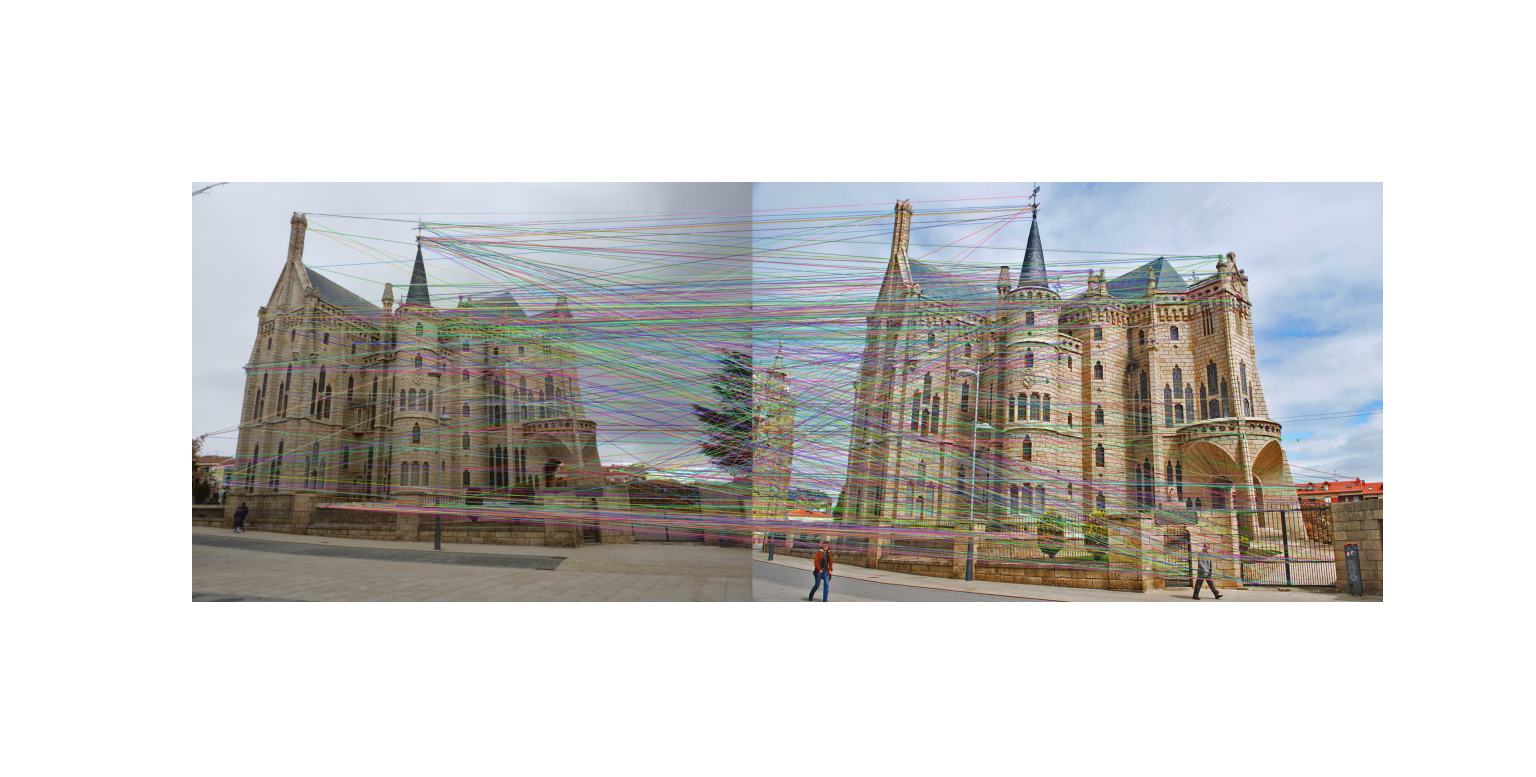
\includegraphics[width=14cm]{images/part3/orb_image_3_0.png}
\end{figure}
\begin{figure}[H]
    \centering
    \includegraphics[width=14cm]{images/part3/orb_image_3_1.png}
\end{figure}


\end{document}

